\documentclass[12pt]{article}
\usepackage[usenames, dvipsnames, table]{xcolor}
\usepackage[utf8]{inputenc}
\usepackage[T1]{fontenc}
\usepackage{lmodern}
\usepackage{amsmath}
\usepackage{amsfonts}
\usepackage{comment}
\usepackage{wrapfig}
\usepackage{booktabs}
\usepackage{tikz}
\usepackage{gnuplottex}
\usepackage{epstopdf}
\usepackage{marginnote}
\usepackage{float}
\usetikzlibrary{tikzmark}
\usepackage{graphicx}
\usepackage{cancel}
\usepackage{bm}
\usepackage{hyperref}

\DeclareMathOperator{\sech}{sech}
\DeclareMathOperator{\csch}{csch}
\DeclareMathOperator{\arcsec}{arcsec}
\DeclareMathOperator{\arccot}{arcCot}
\DeclareMathOperator{\arccsc}{arcCsc}
\DeclareMathOperator{\arccosh}{arcCosh}
\DeclareMathOperator{\arcsinh}{arcsinh}
\DeclareMathOperator{\arctanh}{arctanh}
\DeclareMathOperator{\arcsech}{arcsech}
\DeclareMathOperator{\arccsch}{arcCsch}
\DeclareMathOperator{\arccoth}{arcCoth} 

\newif\ifquoteopen
\catcode`\"=\active % lets you define `"` as a macro
\DeclareRobustCommand*{"}{%
   \ifquoteopen
     \quoteopenfalse ''%
   \else
     \quoteopentrue ``%
   \fi
}

\PassOptionsToPackage{table}{xcolor}

\usepackage{soul}

\newcommand{\hlc}[2]{%
  \colorbox{#1!50}{$\displaystyle#2$}}


\usepackage[a4paper,
            total={170mm,257mm},
 left=20mm,
 top=20mm]{geometry}

\newcommand{\q}[1]{``#1''}
\newcommand{\lamb}[2]{\Lambda^{#1}_{\>{#2}}}
\newcommand{\norm}[1]{\left\lVert#1\right\rVert}
\usepackage{fancyhdr}
\pagestyle{fancy}
\fancyhead{} % clear all header fields
\renewcommand{\headrulewidth}{0pt} % no line in header area
\fancyfoot{} % clear all footer fields
\fancyfoot[LE,RO]{\thepage}           % page number in "outer" position of footer line
\fancyfoot[RE,LO]{Francesco Manzali, Giugno 2018} % other info in "inner" position of footer line

\begin{document}
%Impostazioni booktab (Rimuove quello spazio odioso tra righe)
\setlength{\aboverulesep}{0pt}
\setlength{\belowrulesep}{0pt}
\setlength{\extrarowheight}{.75ex}
\begin{center}
		\line (1,0){350} \\
		[0.25in]
		\huge{\bfseries Fisica moderna}\\
		[2mm]
		\line (1,0){350} \\
		[0.5cm]
		\textsc{\LARGE Relatività}\\
		\textsc{\normalsize Anno accademico 2017-2018}\\ 

	\end{center}

\newgeometry{inner=20mm,
            outer=50mm,% = marginparsep + marginparwidth 
                       %   + 5mm (between marginpar and page border)
            top=20mm,
            bottom=25mm,
            marginparsep=5mm,
            marginparwidth=40mm,
            showframe}
            
\tableofcontents 
\clearpage
\section*{Introduzione}
Buonsalve!\\
In questo documento ho cercato di riordinare gli appunti di Relatività Speciale tratti dal corso di Fisica Moderna tenuto dal professor Flavio Seno presso il Dipartimento di Fisica dell'Università di Padova nel corso del secondo semestre del 2018.\\
Tale lavoro è frutto di una rielaborazione personale, motivata principalmente dall'interesse per la materia\footnote{Fisica moderna is best fisica}. Per questo in diversi punti mi sono concentrato sul ricercare una qualche sorta di \textit{intuizione} per spiegare/visualizzare i risultati ottenuti. Chiaramente non posso garantire che i ragionamenti che ne sono scaturiti siano corretti, ma solo che quando li ho scritti mi sembravano ragionevoli.\\
Potrebbero esserci errori di formattazione, parentesi saltate, o peggio, coefficienti/esponenti/segni errati in giro (ma non dovrebbero essere tanti). Se ne sgamate qualcuno, fatemi sapere. Ditemi anche (se avete tempo e non vi scoccia) se ci sono passaggi non chiari: sono dell'idea che eventuali punti oscuri siano sintomo di qualche cosa che non ho veramente capito (ma che penso di sapere, cosa che è pericolosissima).\\
Per il resto questa non è la versione finale degli appunti: comprende infatti solo gli argomenti dalla cinematica relativistica in poi. Sto ultimando una discussione anche della parte iniziale, che è stata notevolmente rallentata dal cercare di chiarire il significato di componenti covarianti/contravarianti\footnote{Il mio dubbio principale è stato: "E queste chi le ha ordinate?"} e che, eventualmente, aggiungerò qui. Ma poiché le altre parti sono relativamente\footnote{Pun intended} complete, perché aspettare? Magari a qualcuno può servire tutto ciò.\\
Prima di iniziare, ultimo disclaimer (che dovrebbe essere scontato dato che non ho una laurea): questi appunti non sono da intendere come sostituzione delle lezioni, o di altre dispense già presenti.\\
Buon viaggio! :)

\begin{flushright}
\textit{Francesco Manzali}, 03/06/2018
\end{flushright}
\section*{Aggiornamenti}
\begin{table}[hb]
    \centering
    \begin{tabular}{|cccc|}\toprule
        Data & Aggiunte & Errata corrige & Commenti\\\midrule
        \textbf{03/06/2018} & Prima pubblicazione & & \\\bottomrule
    \end{tabular}
    \caption{Cronologia di modifiche/aggiornamenti agli appunti}
    \label{updates}
\end{table}

\clearpage
\begin{comment}



\section{Equazioni di Maxwell e trasformazioni di Galileo}


\section{Trasformazioni di Lorentz} %E diagrammi di Minkowski


Sistema di riferimento: terna di assi cartesiani dotata di orologi identici e sincronizzati \textit{posti in ogni punto dello spazio}. 
Un sdr inerziale è tale che ogni corpo libero (non soggetto a interazioni) è a riposo rispetto ad esso o in moto rettilineo uniforme. Le leggi della fisica sono più \textit{semplici} nei sdr inerziali.
Come sincronizzare gli orologi?
Non si può trasportare un orologio tra due punti (il moto potrebbe cambiarne il funzionamento). Un'altra idea è usare un segnale.
Se fosse possibile un segnale istantaneo ($v = \infty$) il problema sarebbe risolto: basta mandare un segnale da $1$ a $2$, e ricevere come risposta il tempo misurato da $2$, per poi settare il proprio orologio a quel tempo.
Ma la luce (massima velocità) ha una velocità finita, perciò mentre ricevo il segnale da $2$, l'orologio in $2$ continua ad andare avanti, e se imposto l'orologio in $1$ all'ora ricevuta otterrò un orologio "indietro" rispetto a $2$.

Procedura di Einstein. Supponiamo che la luce abbia la stessa velocità tra $1$ e $2$, e tra $2$ e $1$. Tale postulato dà una \textit{definizione operativa del tempo}. Allora due orologi sono sincronizzati se, inviando un segnale da $1$ a $t=0$, la risposta di $2$, ricevuta da $1$ all'istante $t$, è pari a $t/2$. Cioè il segnale impiega $t/2$ a raggiungere $2$, che perciò ci comunica $t/2$, e mentre torna $1$ continua ad andare avanti e arriva a $t/2+t/2=t$.
Procedura di sincronizzazione: siano $1$ e $2$ separati da una distanza $L$ nota. $1$ invia un segnale a $2$, $2$ quando riceve setta il tempo a $t=L/c$. 
Oppure si mette la sorgente alla stessa distanza da $1$ a $2$, e quando $1$ e $2$ vedono il segnale (eventi che postuliamo essere simultanei), allora settano il tempo a $t$ concordato in precedenza.
In altre parole la definizione operativa del tempo si basa sul concetto di \textbf{simultaneità}.

\textbf{Postulati}
\begin{enumerate}
    \item \textbf{Principio di relatività}: Le leggi fisiche hanno la \textbf{stessa forma} in tutti i sistemi di riferimento inerziali
    \item \textbf{Costanza di $c$}: La velocità della luce nel vuoto ha lo stesso valore in tutti i sistemi di riferimento inerziali.
\end{enumerate}

\end{comment}
\section{Cinematica relativistica}
\subsection{Decadimenti}
In un decadimento una particella si \textit{scompone} spontaneamente in più particelle diverse. Si tratta di un fenomeno probabilistico, per cui non è possibile determinare in anticipo quando una data particella decadrà.
\marginpar{Equazione dei decadimenti}
Tuttavia, considerando quantità macroscopiche di sostanze, è possibile scrivere una legge statistica riguardante il decadimento:
\[
N(t+dt) = N(t) - \lambda N(t) dt \Rightarrow \frac{dN}{N} = -\lambda
\]
$N(t)$ è il numero di particelle della sostanza iniziale presenti nel sistema considerato al tempo $t$. Dopo un intervallo infinitesimo $dt$, tale numero è destinato a decrescere con una velocità $\lambda$, che costituisce la \textit{costante di decadimento}. La soluzione esplicita dell'equazione differenziale è:
\[
N(t) = N_0 e^{-\frac{t}{\tau}}; \quad \tau = \frac{1}{\lambda}
\]
dove $\tau$ (\textit{vita media}) è l'intervallo di tempo necessario a ridurre la popolazione iniziale $N_0$ di particelle al $36.8\%$ ($1/e$). Spesso si fa ricorso al \textbf{tempo di dimezzamento} $t_{1/2} = \ln 2 \tau$, che corrisponde all'intervallo medio di tempo necessario perché il numero iniziale di particelle si dimezzi.\\
\marginpar{Massa iniziale $\geq$ massa prodotti}
Si consideri un generico urto in cui una particella di massa $M$ si scompone in $N$ particelle di masse $m_1 \dots m_N$.\\
Poniamoci nel sistema di riferimento in cui la particella iniziale è ferma, che da ora in poi chiameremo \textit{sdr} del centro di massa (CM). Allora, ponendo $c = 1$, si avrà che:
\[
p^\mu p_\mu = p^{{*,0}^2}-|\cancel{\bar{p}^*}|^2 = M^2 \Rightarrow p^{*,0} = M
\]
%Perché abbiamo fatto questo conto? [TO DO]
Applicando la conservazione dell'energia:
$$M = E_1^* + \dots + E_N^* = \sum_{i=1}^{N} E_i^* = \sum_{i=1}^N \sqrt{m_i^2+p_i^{*,2}} \geq \sum_{i=1}^N m_i$$ 
ossia la somma delle masse delle particelle prodotte dal decadimento deve essere minore della massa iniziale della particella che si è decomposta (non si può creare massa dal nulla).\\
\marginpar{Decadimento in due particelle}
Si consideri ora una particella di massa $M$ che decade in \textbf{due} particelle più piccole di massa $m_1$ e $m_2$, con $M$ che è inizialmente in movimento rispetto al sdr del laboratorio.\\
In questo caso è conveniente analizzare il moto nel sdr del centro di massa del sistema (la cui origine coincide ovviamente con la particella iniziale), indicato con $*$.\\
Nel sdr del CM il trimomento iniziale è nullo, e perciò, indicati con $\bar{p}^*_1$ e $\bar{p}^*_2$ i trimomenti delle particelle prodotte, si avrà:
\begin{equation}
\bar{p}_1^* + \bar{p}_2^* = 0 \Rightarrow |\bar{p}^*_1| = |\bar{p}^*_2| = p^*
\label{momenti}
\end{equation}
ossia le particelle prodotte hanno, in modulo, lo stesso trimomento, e sono lanciate lungo la stessa direzione in versi opposti.\\
Detto $\theta^*$ l'angolo descritto con $+\hat{x}$ dal moto della prima particella prodotta, si ha perciò:
\[
p_1^* = \left (\frac{E_1^*}{\cancel{c}}, p^*\cos\theta^*, p^*\sin\theta^*,0 \right ); \quad p_2^*=(E_2^*, -p^*\cos\theta^*, -p^*\sin\theta^*, 0)
\]
Nota: da qui in poi si userà la convenzione per cui $c = 1$.\\
Ricavando le energie dai momenti:
\begin{equation}
    E_1^{*^2}  = m_1^2  \cancel{c^4} + p^{*^2}\cancel{c^2}; \quad E_2^{*^2} = m_2^2 + p^{*^2} \Rightarrow \hlc{SkyBlue}{E_1^{*^2}-E_2^{*^2} = m_1^2-m_2^2}
    \label{diff-energie}
\end{equation}

Applicando la conservazione dell'energia nel sdr del CM (dove la particella iniziale è ferma):
\begin{equation}
\hlc{Yellow}{M\cancel{c^2} = E_1^* + E_2^*} \Rightarrow E_1^* = M-E_2^*
\label{cons-energia}
\end{equation}
Possiamo ora mettere a sistema \ref{diff-energie} e \ref{cons-energia} per ricavare le energie in funzione delle masse. La via più veloce è moltiplicando e dividendo per l'\textcolor{ForestGreen}{energia totale}:
\marginpar{Energia e momento}
\begin{align}
(E_1^* - E_2^*) \frac{\textcolor{ForestGreen}{E_1^*+E_2^*}}{\textcolor{ForestGreen}{E_1^* + E_2^*}} &=
\frac{ \hlc{SkyBlue}{E_1^{*^2}-E_2^{*^2}} }{\hlc{yellow}{E_1^* + E_2^*}} =
\frac{m_1^2-m_2^2}{M} = M-2E_2^*\\
&\Rightarrow 
\begin{cases}
E_1^* = \displaystyle\frac{M^2-m_2^2+m_1^2}{2M}\cancel{c^2}\\
E_2^* = \displaystyle\frac{m_2^2-m_1^2+M^2}{2M}\cancel{c^2}
\label{Energie}
\end{cases}
\end{align}
Da \ref{diff-energie} si ricava $p^{*^2} = E_1^{*^2} - m_1^2$, e sostituendo l'espressione appena trovata per $E_1^{*^2}$ si giunge a:
\begin{equation}
    p^{*^2} = \frac{1}{4M^2}[M^4 + m_1^4 + m_2^4 -2M^2(m_1^2+m_2^2)-2m_1^2 m_2^2]
    \label{momentoquadro}
\end{equation}

Chiamiamo $\theta^*_\alpha$ \marginpar{Angolo} l'angolo formato dalla velocità della particella di massa $m_\alpha$ (con $\alpha = 1,2$, poiché il decadimento è in due particelle) con l'asse $+\hat{x}$ appena dopo il decadimento. Scomponendo la quantità di moto sugli assi si ottiene $p^*_{\alpha,x} = p^* \cos\theta_\alpha^*$ e $p_{\alpha,y}^* = p^* \sin\theta_\alpha^*$. Nel sdr del CM, si avrà poi $\theta_2^* = \pi - \theta_1^*$, in quanto i momenti delle due particelle sono opposti.\\
Nel sdr del laboratorio, tuttavia, la particella iniziale è in movimento, e perciò la direzione di uscita delle particelle del decadimento non sarà opposta, ma tale che il momento (inizialmente non nullo) sia conservato.\\
Applicando la trasformazione di Lorentz al quadrimomento si ottiene:
\[
p_\alpha = \begin{bmatrix}\gamma & \beta\gamma & 0 & 0\\ \beta\gamma & \gamma & 0 & 0\\
0 & 0 & 1 & 0\\ 0 & 0 & 0 & 1
\end{bmatrix} \begin{bmatrix} 
E_\alpha^*/\cancel{c} \\ p^*\cos \theta_\alpha^* \\ \hlc{Green}{p^*\sin \theta_\alpha^*}\\ 0
\end{bmatrix} = 
\begin{bmatrix}
\gamma(E_\alpha^* + \beta p^* \cos\theta_\alpha^*) \\
\gamma(p^*\cos\theta_\alpha^* + \beta E_\alpha^*)\\
\hlc{Green}{p^*\sin\theta_\alpha^*}\\
0
\end{bmatrix} = 
\begin{bmatrix}
E_\alpha/\cancel{c}\\
p_{\alpha,x}\\
p_{\alpha,y}\\
p_{\alpha,z}
\end{bmatrix}
\]
Scrivendo il quadrato del momento $p^*$ in funzione di $p_{\alpha,x}$ e $p_{\alpha,y}$ si giunge a:
\[
\left ( \frac{p_{\alpha,x}}{\gamma} -\beta E_\alpha^* \right )^2 + p_{\alpha,y}^2 = p^{*^2} (\cos^2\theta_\alpha^* + \sin^2\theta_\alpha^*) = p^{*^2}
\]
Equazione che può essere riarrangiata come:
\begin{equation}
\frac{(p_{\alpha,x} - \hlc{Yellow}{\gamma\beta E_\alpha^*} )^2}{(\hlc{SkyBlue}{p^* \gamma})^2} + \frac{p_{\alpha,y}^2}{\hlc{ForestGreen}{p^{*^2}}} = 1
\label{ellisse}
\end{equation}
che rappresenta un'ellisse sul piano $p_{\alpha,x},\, p_{\alpha,y}$, con centro posto a $(\hlc{Yellow}{\gamma\beta E_\alpha^*}, 0)$ e semiassi $s_x = \hlc{SkyBlue}{p^*\gamma}$ e $s_y = \hlc{ForestGreen}{p^*}$
%[TO DO] Grafico dell'ellisse
In particolare l'ellisse può non comprendere l'origine se il centro si trova ad una distanza dall'origine maggiore della lunghezza del semiasse $s_x$, ossia per $\beta > p^* / E_\alpha^* = \beta_{\alpha}^*$, dove $\beta = v_{CM}/c$ (nel sdr del laboratorio). Quando ciò si verifica si parla di \textbf{emissione in avanti}.

Per determinare \marginpar{Angolo massimo} il valore dell'angolo massimo, consideriamo una retta generica sul piano $p_{\alpha,x},\,p_{\alpha,y}$, che sarà parametrizzata come $p_{\alpha,x} = q\sin\theta$, da cui $p_{\alpha,y} = q\cos\theta$. Intersecando l'equazione \ref{ellisse} con tale retta, e imponendo la condizione di $\Delta = 0$ nell'equazione di secondo grado risultante, è possibile determinare il valore di $\theta_{max}$ per cui la retta risulta tangente all'ellisse.\\
Ponendo $\epsilon' = \beta E_\alpha^*$ per semplicità, ed effettuando le sostituzioni, si ottiene:
\[
\frac{(q\cos\theta -\gamma\epsilon ' )^2}{\gamma^2} + q^2\sin^2\theta = p^{*^2}
\]
Dalla relazione $\gamma^2 = 1/(1-\beta^2)$ e svolgendo il quadrato si giunge a:
\[
q^2 \cos^2\theta (1-\beta^2) + \epsilon'^2 - \frac{2q\cos\theta \epsilon '}{\gamma} + q^2\sin^\theta = p^{*^2}
\]
Raccogliendo un $q^2$ e semplificando si giunge infine a:
\[
q^2(1-\beta^2\cos^2\theta) - \frac{2q \cos\theta\epsilon '}{\gamma} + \epsilon'^2 - p^{*^2} = 0
\]
Con $A = 1-\beta^2 \cos^2\theta$, $B = \cos\theta\epsilon ' /\gamma$ e $C = \epsilon'^2 - p^{*^2}$ si evidenzia l'equazione di secondo grado: $q^2 A - 2qB + C = 0$. Imponendo il $\Delta = 0$ si ha:
\[
B^2-AC = 0 = \cos^2\theta \epsilon'^2 (1- \cancel{\beta^2}) - (\epsilon'^2-p^{*^2}) + \beta^2\cos^2\theta (\cancel{\epsilon'^2} - p^{*^2}) = 0
\]
Espandendo si ottiene l'espressione per il coseno:
\[
\cos^2\theta (\epsilon'^2 - p^{*^2}\beta^2) = \epsilon'^2 - p^{*^2} \Rightarrow \cos^2\theta = \frac{\epsilon'^2-p^{*^2}}{\epsilon'^2-p^{*^2}\beta^2}
\]
Da cui si può ottenere quella per il seno tramite $\sin^2 \theta = 1-\cos^2\theta$:
\[
\sin^2 \theta = \frac{p^{*^2} (1-\beta^2) }{\hlc{Yellow}{\epsilon'^2-p^{*^2}\beta^2}}
\]
È possibile riscrivere il denominatore partendo dalla relazione:
\[
E^2 = m^2 + p^2 \Rightarrow m_\alpha = \hlc{SkyBlue}{E_\alpha^2} - p^{*^2} = \frac{\epsilon'^2}{\beta^2} - p^{*^2} = \frac{\epsilon'^2 - p^{*^2}\beta^2}{\beta^2} \Rightarrow \hlc{Yellow}{m_\alpha\beta^2} = \epsilon'^2-p^{*^2}\beta^2
\]
dove si è sfruttata la sostituzione $\epsilon'^2 = \beta^2 E_\alpha^2 \Rightarrow E_\alpha^2 = \hlc{SkyBlue}{\epsilon'^2/\beta^2}$. Si giunge perciò ad un'espressione più semplice per il seno:
\[
\sin^2\theta = \frac{p^{*^2}(1-\beta^2)}{m_\alpha^2\beta^2} = \frac{p^{*^2}}{m_\alpha^2 \beta^2\gamma^2} \Rightarrow \sin\theta_\alpha^{max} = \frac{p^{*}}{m_\alpha\beta\gamma}
\]

Se la particella \marginpar{Distribuzione delle energie}che decade ha uno \textit{spin} nullo, allora, nel sistema di riferimento del centro di massa, la distribuzione degli angoli d'uscita delle particelle generate sarà uniforme: non ci sarà cioè un angolo d'uscita \textit{più probabile} degli altri, e le particelle saranno emesse equamente in ogni direzione. Partendo da questo fatto sperimentale, ci si pone il problema di determinare la distribuzione delle energie delle particelle osservata nel sistema di riferimento del laboratorio, rispetto al quale il CM si muove a velocità $v$, da cui sono determinati i parametri $\beta$ e $\gamma$.\\
Consideriamo un certo numero $M$ di decadimenti, che produrrà $N_{tot}$ particelle risultanti. Ponendo un rilevatore sferico attorno al sito di decadimento e stazionario rispetto ad esso (quindi stazionario nel sdr del CM), ci si aspetta che attraverso sezioni uguali di rilevatore passi (mediamente) lo stesso numero di particelle. In altre parole il numero di particelle $N'$ che passa attraverso una certa sezione $A$ è proporzionale all'area di tale sezione tramite una costante che chiamiamo $\sigma$: $N(A) = \sigma A$, con $\sigma = N_{tot}/4\pi$. Poiché abbiamo usato una sfera di raggio unitario, $A$ corrisponde (per definizione) all'angolo solido sotteso da quella sezione (da $\Omega = A/r^2$, con $r=1$).\\
Fissato un sistema di coordinate sferiche attorno al CM, con angoli $\theta$ e $\varphi$, possiamo ora costruire la funzione densità di probabilità $d\chi(\theta^*)$ che restituisce la probabilità di una particella di uscire ad un angolo $\theta^*$, ossia di attraversare la \textit{corona sferica} compresa tra $\theta^*$ e $\theta^*+d\theta^*$. Tale sezione sottende un angolo solido pari a:
\[
d\Omega^* = (2\pi\sin\theta^*)d\theta^*
\]
(Basta figurarsi la sfera unitaria: $2\pi\sin\theta^*$ è la circonferenza \textit{interna} della corona sferica, e $d\theta$ è il suo \textit{spessore} infinitesimo. \textit{Srotolando la striscia della corona circolare essa risulta un rettangolo dalle cui dimensioni ricaviamo l'area}).\\
Sostituendo nell'espressione per $N(\Omega)$:
\[
dN(\Omega) = \sigma d\Omega \Rightarrow dN(\theta^*) = \left ( \frac{N_{tot}}{4\pi}\right ) (2\pi \sin\theta^* d\theta^*)
\]
$dN(\theta^*)$ è perciò il numero di particelle, originate da $M$ decadimenti, con angolo di uscita pari a $\theta^*$ nel sdr del CM. Per giungere alla densità di probabilità cercata, è necessario normalizzare: basta dividere per il numero di particelle originate ($N_{tot}$):
\[
dN(\theta^*) = \frac{1}{2}\sin\theta^* d\theta^* = \frac{1}{2}d\cos\theta^*
\]
$dN(\theta^*)$ è la probabilità, e $f(\theta^*)=\frac{1}{2}\sin\theta^*$ è la \textit{funzione densità di probabilità}. Nel secondo passaggio è sottinteso un cambio di variabile casuale da $\theta^*$ a $\cos\theta^*$: il segno $-$ che comparirebbe di norma è cancellato dal modulo della formula del cambio di variabili casuali (in quanto una pdf è definita positiva): vedi appendice.\\
Poiché ci interessa effettuare un cambio di variabile per associare angoli ad energie (e ricavare la distribuzione delle energie), conviene adottare come variabile direttamente $\cos\theta^*$. Il cambio di variabile è infatti dato dalla trasformazione di Lorentz dell'energia:
\[
E(\cos\theta^*) = \gamma(E^* + \beta p^* \hlc{Yellow}{\cos\theta^*})
\]
Prendendo quindi la funzione densità di probabilità $f(\cos\theta^*) = 1/2$ (ricavata sopra), si può applicare direttamente la \textit{formula per il cambio di variabile casuale}:
\[
\rho(E) = \frac{f(E(\cos\theta^*))}{\left |\displaystyle\frac{d}{d\cos\theta^*} E(\cos\theta^*) \right |} = \frac{1/2}{\displaystyle\frac{d}{d\cos\theta^*} \gamma(E^* + \beta p^* \cos\theta^*)} = \frac{1}{2\gamma\beta p^*}
\]
Alternativamente, per andare veloci, si può usare il metodo (barbaro) di moltiplicare i differenziali:
\[
\rho(E) = \frac{d\chi(E(\theta^*))}{dE} = \underbrace{\frac{d\chi(E(\theta^*))}{d\cos\theta^*}}_{1/2} \underbrace{\frac{d\cos\theta^*}{dE}}_{1/(\gamma\beta p^*)} = \frac{1}{2}\frac{1}{\gamma\beta p^*} 
\]
In ogni caso, $\rho(E)$ è la pdf delle energie delle particelle generate dal decadimento di una particella con spin nullo. Essa è definita nel dominio costituito dall'intervallo $[E_{min}, E_{max}]$, con $E_{min} = \gamma(E^* \bm{-} \beta p^*)$ e $E_{max} = \gamma(E^* \bm{+} \beta p^*)$.\\
Verifichiamo che sia ben definita, ossia che l'integrale sul suo dominio sia pari a $1$:
\[
\int_{E_{min}}^{E_max} \rho(E)dE = \int_{E_{min}}^{E_max} \frac{1}{2\gamma\beta p^*}dE = \frac{1}{2\gamma\beta p^*}(E_{max}-E_{min}) = \frac{1}{2\gamma\beta p^*}(\gamma\beta p^* + \gamma\beta p^*) = 1
\]

Consideriamo ora il caso speciale di un decadimento \marginpar{Decadimento in due masse uguali} in due masse uguali: $M \to m + m$.\\
Riscrivendo le equazioni \ref{momenti}, \ref{Energie}, \ref{momentoquadro} con $m_1 = m_2 = m$:
\begin{equation}
    \bar{p}_1^* + \bar{p}_2^* = 0; \quad |p_1^*| = |p_2^*| := p^* = \sqrt{\frac{M^2}{4}-m^2}; \quad E_1^* = E_2^* = \frac{M}{2} := E^*
\end{equation}
Da cui: 
\begin{equation*}
    \beta_1^* = \beta_2^* = \frac{p^*}{E^*} = \frac{2p^*}{M} := \beta^*
\end{equation*}
Sia ora $\theta_\alpha^*$ l'angolo d'uscita della particella $\alpha$-esima nel sdr del CM. Scomponendo la quantità di moto lungo gli assi e passando al sdr del laboratorio si giunge a:
\[
p_{\alpha,x} = \gamma(p^*\cos\theta_\alpha^* + \beta E^*); \quad p_{\alpha y} = p^*\sin\theta_\alpha^*
\]
Da cui:
\[
\tan\theta_\alpha = \frac{p_{\alpha y}}{p_{\alpha x}} = \frac{p^* \sin\theta_\alpha^* }{\gamma(p^*\cos\theta_\alpha^* + \beta E^*)} = \frac{\sin\theta_\alpha^*}{\gamma \displaystyle \left ( \cos\theta_\alpha^* + \beta \hlc{Yellow}{\frac{E^*}{p^*}} \right )} \underset{(*)}{=} \frac{\sin\theta_\alpha^*}{\displaystyle \gamma\left ( \cos\theta_\alpha^* + \frac{\beta}{\beta^*} \right )}
\]
In $(*)$ si effettuata la sostituzione $\beta^* = p^*/E^* \Rightarrow \hlc{Yellow}{1/\beta^*} = E^*/p^*$.\\
Definendo l'angolo $\theta^* = \theta_1^*$, poiché le due masse sono emesse lungo la stessa direzione in versi opposti (nel sdr del CM), valgono le relazioni:
\[
\sin\theta_1^* = -\sin\theta_2^* := \sin\theta^*; \quad \cos\theta_1^* = - \cos\theta_2^* = \cos\theta^*
\]
Da cui:
\begin{equation}
\tan \theta_1 = \frac{\sin\theta^*}{\gamma\left (\cos\theta^* \bm{+} \displaystyle\frac{\beta}{\beta^*} \right )};\quad
\tan \theta_2 = 
\frac{-\sin\theta^*}{\gamma\left (-\cos\theta^* \bm{+} \displaystyle\frac{\beta}{\beta^*}  \right )} = 
\frac{\sin\theta^*}{\gamma\left (\cos\theta^* \bm{-} \displaystyle\frac{\beta}{\beta^*} \right )}
    \label{tangenti}
\end{equation}
Consideriamo ora l'angolo $\theta = \theta_1-\theta_2$ formato dalle direzioni d'uscita delle due particelle (nel sdr del laboratorio). \marginpar{Angolo tra le particelle} La formula di sottrazione delle tangenti è data da:
\[
\tan\theta = \tan(\theta_1-\theta_2) = \frac{\tan\theta_1 - \tan\theta_2}{1+\tan\theta_1\tan\theta_2}
\]
e applicandola alle tangenti in \ref{tangenti}:
\begin{align*}
    \tan\theta &= \frac{
    \displaystyle \frac{\sin\theta^*}{\gamma \left ( \cos\theta^* + \frac{\beta}{\beta^*} \right ) } + \frac{\sin\theta^*}{\gamma\left (\cos\theta^* \bm{-} \displaystyle\frac{\beta}{\beta^*} \right ) }
    }{ \displaystyle
    1 + \frac{\sin^2\theta^*}{\gamma^2 \left ( \cos^2\theta - \frac{\beta}{\beta^*} \right )}
    } =
    \frac{\displaystyle
        \frac{
            \cancel{\sin\theta^*\cos\theta^*} - \frac{\beta}{\beta^*}\sin\theta^* - \cancel{\sin\theta^*\cos\theta^*} - \frac{\beta}{\beta^*}\sin\theta^*
        }{
        \hlc{SkyBlue}{\gamma \left (\cos^2\theta^* - \frac{\beta^2}{\beta^{*^2}} \right )}
        }
    }{\displaystyle
        \frac{
            \gamma^2 \left ( \cos^2\theta^* - \frac{\beta^2}{\beta^{*^2}} \right ) + \sin^2\theta^*
        }{
            \hlc{SkyBlue}{\gamma^2 \left ( \cos^2\theta^* - \frac{\beta^2}{\beta^{*^2}} \right )}
        }
    } = \\
    & = \frac{\displaystyle
        -\frac{2\beta\sin\theta^*}{\beta^*}\gamma
    }{\displaystyle
        \gamma^2 \left [ \hlc{Yellow}{\cos^2\theta^*} - \frac{\beta^2}{\beta^{*^2}} + \hlc{Yellow}{\sin^2\theta^*(1}-\beta^2) \right ] 
    } = %\gamma^2 al denominatore!? dove sparisce?
    \frac{\displaystyle
    -\frac{2\beta}{\beta^* \gamma}\sin\theta^*
    }{\displaystyle
    \left [ 1 - \frac{\beta^2}{\beta^{*^2}} - \beta^2\sin^2\theta^* \right ]
    } = \\
    & = 
    \frac{\displaystyle
    \cancel{-}\frac{2\beta}{\beta^* \gamma}\sin\theta^*
    }{
    \cancel{-}\beta^2 \left [ -\frac{1}{\beta^2} + \frac{1}{\beta^{*^2}} + \sin^2\theta^* \right ]
    } = 
    \frac{\displaystyle
        \frac{2}{\beta\beta^*\gamma}\sin\theta^*
    }{\displaystyle
        \sin^2\theta^* + \frac{1}{\beta^{*^2}} - \frac{1}{\beta^2}
    } := f(\theta^*)\>\square
\end{align*}
che riscriviamo per semplicità come:
\[
f(\theta^*) = \tan\theta = \frac{A\sin\theta^*}{\sin^2\theta^* + B}; \quad \begin{cases}
A = \displaystyle \frac{2}{\beta \beta^* \gamma}\\
B = \displaystyle \frac{1}{\beta^{*^2}} - \frac{1}{\beta^2}
\end{cases}
\] 
Passiamo ora allo \textit{studio} della funzione $f(\theta^*)$.\\
Il denominatore si annulla per $\sin^2\theta^* = -B$, che ha soluzione solo per $-1<B<0$, dove si avrà $\theta^* = \arcsin (\pm \sqrt{-\beta})$. La funzione si annulla per $\sin\theta^* = 0$, ossia per $\theta^* = 0,\pi$ (definendo $\theta^*$ tra $0$ e $\pi$, e quindi ignorando la periodicità).\\ %[TO DO] Controllare definizione dell'angolo \theta^*
Calcoliamo le derivate prima e seconda:
\begin{align}
    f'(\theta^*) &= \frac{
    A\cos\theta^* (B-\sin^2\theta^*)
    }{
    (B+\sin^2\theta^*)^2
    }
    \label{derivata-prima}\\
    f''(\theta^*) &= -\frac{
    A\sin\theta^*
    }{
    (B+\sin\theta^*)^3
    } \left [
    B^2 +6B\cos^2\theta^* -2\sin^2\theta^*\cos^2\theta^* -\sin^4\theta^*
    \right ]
    \label{derivata-seconda} 
\end{align}
Cerchiamo ora i punti stazionari. La derivata prima si annulla quando $\cos\theta^* = 0$, ossia per $\theta^* = \pi/2$, oppure quando $B = \sin^2\theta^*$, cosa che succede solo per $0 < B < 1$. Concentriamoci sul primo caso.\\
Detto $\bar{\theta}$ (sdr laboratorio) il valore per cui si ha $\theta^* = \pi/2$ (sdr del CM), calcoliamo il valore che la funzione assume in tale punto:
\begin{align*}
\tan\left (\theta \left (\frac{\pi}{2} \right ) \right ) &= \tan(\bar{\theta}) = \frac{A}{1+B} =
\frac{\displaystyle
\frac{2}{\beta\beta^*\gamma}
}{\displaystyle
1+\left (\frac{1}{\beta^{*^2}}-\frac{1}{\beta^2}\right )
} = 
\frac{\displaystyle
\frac{2}{\hlc{SkyBlue}{\beta\beta^*}\gamma}
}{\displaystyle
\frac{\beta^{*^2}\beta^2 + \beta^2 - \beta^{*^2}}{\hlc{SkyBlue}{\beta^{*^2}\beta^2}}
} =\\
& =
\frac{
2\beta^*\beta
}{
\gamma(\beta^2-\beta^{*^2}+\beta^{*^2}\beta^2)
} \underset{/\beta^2}{=} 
\frac{
2\beta^*
}{
\gamma\beta \displaystyle \frac{\beta^2 - \beta^{*^2}\hlc{Yellow}{(1-\beta^2)}}{\beta^2}
} \underset{(*)}{=} 
\frac{
2\beta^*
}{\displaystyle
\gamma\beta \left ( 1 - \frac{\beta^{*^2}}{(\gamma\beta)^2} \right )
}
\end{align*}
dove in $(*)$ si è usata la sostituzione $\hlc{Yellow}{1/\gamma^2} = (1-\beta^2)$, per poi spezzare la frazione e giungere al risultato finale.
Notiamo che, poiché $A \geq 0$ per definizione, il segno di $\tan\bar{\theta}$ è determinato da quello di $B$, tramite:
\[
\begin{cases}
B < -1 & \Leftrightarrow \tan\bar{\theta} < 0\\
B > -1 & \Leftrightarrow \tan\bar{\theta} > 0
\end{cases}
\]
In particolare $B < -1$ se:
\[
\frac{1}{\beta^{*^2}}-\frac{1}{\beta^2} < -1 \Rightarrow \beta^2 - \beta^{*^2} < -\beta^2\beta^{*^2} \Rightarrow -\beta^{*^2}(1-\beta^2) < -\beta^2 \Rightarrow \beta^2 < \frac{\beta^{*^2}}{\gamma^2} \Rightarrow \beta < \frac{\beta^{*}}{\gamma}
\]
E per $B = -1$ si ha $\beta = \beta^*/\gamma$.
\\
Si può semplificare la formula ottenuta per $\tan\bar{\theta}$ ricordando la formula di duplicazione della tangente:
\begin{equation}
    \tan\alpha = \frac{\displaystyle 2\tan\frac{\alpha}{2}}{1-\displaystyle\tan^2\frac{\alpha}{2}}
    \label{duptangente}
\end{equation}
E osservando che il risultato per $\tan\bar{\theta}$ ha la stessa formula del secondo membro di \ref{duptangente}, si ottiene per confronto:
\begin{equation}
\tan \frac{\bar{\theta}}{2} = \frac{\beta^*}{\gamma\beta} \Rightarrow \bar{\theta} = 2\arctan \frac{\beta^*}{\gamma\beta}
\label{thetabarra}
\end{equation}
Verifichiamo la tipologia di estremo calcolando la derivata seconda in $\bar{\theta}$:
\[
f''(\bar{\theta}) = -\frac{A}{(B+1)^3}(B^2-1) = - \frac{A}{(B+1)^2}(B-1)
\]
Di nuovo, il segno dipende solo da $B$, e si ha:
\[
\begin{cases}
B < 1 &\Leftrightarrow f''(\bar{\theta}) > 0 \Rightarrow \bar{\theta} \text{ min }\\
B > 1 &\Leftrightarrow f''(\bar{\theta}) < 0 \Rightarrow \bar{\theta} \text{ max }
\end{cases}
\]
In particolare, $B < 1$ se:
\[
\frac{1}{\beta^{*^2}}-\frac{1}{\beta^2} < 1 \Rightarrow \beta^2 - \beta^{*^2} < \beta^2\beta^{*^2} \Rightarrow \beta^2(1-\beta^{*^2}) < \beta^{*^2} \Rightarrow \frac{\beta^2}{\gamma^{*^2}} < \beta^{*^2} \Rightarrow \beta < \beta^* \gamma^*
\]
e con $B = 1$ si ha $\beta = \beta^*\gamma^*$.\\
Concentriamoci ora sull'altro caso in cui la derivata prima può annullarsi, e cioè quando $B = \sin^2\theta^*$ (che si verifica solo per $0<B<1$). Definiamo l'angolo $\theta_0$ come l'angolo a cui ciò si verifica: $B = \sin^2\theta_0^2$.\\
Il valore della funzione in $\theta_0$ è dato da: %[TO DO] controllare qui i conti
\[
\tan(\theta(\theta_0^*)) = \frac{A\sin\theta_0^*}{2\sin^2\theta_0^*} = \frac{A}{2\sin\theta_0^*} = \frac{1}{\gamma\beta\beta^*\sin\theta_0^*}
\]
Per come abbiamo definito $\theta_0$:
\[
\sin\theta_0^* = \sqrt{\frac{1}{\beta^{*^2}} - \frac{1}{\beta^*}} = \frac{\sqrt{\beta^* - \beta^{*^2}}}{\beta^*\beta} 
\]
E sostituendo nell'espressione di sopra:
\[
\tan\theta_0 = \frac{1}{\gamma\sqrt{\beta^2 - \beta^{*^2}}} \Rightarrow \theta_0 = \arctan \frac{1}{\gamma \sqrt{\beta^2 -\beta^{*^2}}}
\]
Esaminiamo anche qui la tipologia di estremo calcolando la derivata seconda:
\[
f''(\theta_0) = -\frac{A\sin\theta_0^*}{8\sin^2\theta_0^*}(4\sin^2\theta_0^* \cos^2\theta^*) < 0 \Rightarrow \text{$\theta_0$ punto di max}
\]
Riepilogando, ricordando che per $-1 < B < 0$ la funzione presenta asintoti, e che per $B = 0$ si ha $\beta^* = \beta$, vi sono quattro sezioni principali in cui studiare la funzione $\tan\theta$:
\begin{enumerate}
    \item $B < -1$ ($\beta < \beta^*/\gamma$): nessun asintoto, $\bar{\theta}$ è un punto di minimo globale
    \item $-1 < B < 0$ ($\beta^*/\gamma < \beta < \beta^*)$: due asintoti verticali, $\bar{\theta}$ è un punto di minimo locale
    \item $0 < B < 1$ ($\beta^* < \beta < \beta^*\gamma^*$): nessun asintoto, $\bar{\theta}$ è un punto di minimo, mentre $\theta_0$ è massimo globale
    \item $B > 1$ ($\beta > \beta^*\gamma^*$): nessun asintoto, $\bar{\theta}$ è un punto di massimo globale
\end{enumerate}
In tutti i casi la funzione si annulla in $0$ e $\pi$.\\
\subsubsection{Angoli tra particelle: riepilogo e qualche intuizione}
\begin{figure}%
\centering%
    \begin{gnuplot}[terminal=epslatex, terminaloptions=color dashed, terminaloptions={size 17cm,26cm}]
            
            set ylabel " " 
            
            set xrange [0:pi]
            
            
            set mxtics 5
            set mytics 2
            
            
            set xzeroaxis
            
            set xtics format " "
            set xtics 1
            
            set key center bottom
            set key reverse
            
            set style fill pattern 5 border
            set style line 12 lc rgb '#808080' lt 0 lw 1
            set grid back ls 12
            
            set style line 1 lc "blue" lw 2
            set style line 2 lt rgb "#black" lw 1
            set style line 3 lt rgb "#5060D0" lw 2 pt 2
            set style line 4 lt rgb "red" lw 2 pt 9
            
            
            set tmargin 0
            set bmargin 0
            set lmargin 2
            set rmargin 1
            
            beta = 0.5
            betastar = 0.5
            gamma(beta) = 1/sqrt(1-beta*beta)
            A(beta, betastar) = 2/(gamma(beta)*betastar*beta)
            B(beta, betastar) = 1/(betastar*betastar) - 1/(beta*beta)
            f(x) = A(beta,betastar)*sin(x)/(B(beta,betastar)+sin(x)*sin(x))
            
            set multiplot layout 4,2 margins 0.05,0.95,.1,.99 spacing 0,0
            
            #B < -1
            set xtics format " "
            set xtics (0, pi/4, pi/2, 3*pi/4, pi)
            set x2tics ("$0$" 0,"$\\displaystyle\\frac{\\pi}{4}$" pi/4,"$\\displaystyle\\frac{\\pi}{2}$" pi/2, "$\\displaystyle\\frac{3\\pi}{4}$" 3*pi/4, "$\\pi$" pi) offset 0, 0.3
            set x2label "Angolo $\\theta^*$" offset 0, 0.5
            
            set ytics -3.5,0.5,-0.5
            set yrange [-4:0]
            
            beta = 0.4
            betastar = 0.5
            set ylabel "$B < -1$"
            
            set label 1 at pi/2, -0.3 "$\\beta = 0.4;\\>\\beta^* = 0.5; \\> B = -2.25$" center front
            
            plot f(x) title "$\\>\\tan\\theta(\\theta^*)$" ls 1
            
            unset label 1
            unset x2label
            
            set ytics format " "
            unset x2tics
            
            set x2label "Circonferenza goniometrica"
            set parametric
            set key center top
            set xrange [-1.1:1.1]
            set xtics (-1, 0, 1)
            
            set ytics (0, sqrt(2)/2, 1)
            set y2tics ("$0$" 0, " " sqrt(2)/2, "$1$" 1)
            
            set trange [0:pi]
            set yrange [0:1.7]
            unset ylabel
            
            set label 2 at -0.6, 0.16 "$\\displaystyle 2|\\arctan \\frac{\\beta^*}{\\gamma\\beta}|$" center front
            set label 3 at -sqrt(2)/2, sqrt(2)/2 + 0.1 "$\\bar{\\theta}$" center front
            
            fx(t) = cos(t)
            fy(t) = sin(t)
            plot fx(t),fy(t) ls 2 notitle, fx(t/4+3*pi/4),fy(t/4+3*pi/4) lc rgb "red" lw 4 notitle, -t,t notitle,  0.2*fx(t/4+3*pi/4),0.2*fy(t/4+3*pi/4) ls 3 notitle
            
            unset label 2
            unset label 3
            unset x2tics
            unset y2tics
            
            unset parametric
            unset yrange
            unset x2label
            
            #-1 < B < 0
            set xtics (0, pi/4, pi/2, 3*pi/4, pi)
            set xrange [0:pi]
            beta = 0.47
            betastar = 0.5
            set yrange[-150:150]
            set ytics (-100, -50, 0, 50, 100)
            set ytics format "%.0s"
            set key center bottom
            set ylabel "$-1 < B < 0$"
            
            set label 1 at pi/2, 130 "$\\beta = 0.47;\\>\\beta^* = 0.5; \\> B = -0.53$" center front
            
            plot f(x) title "$\\>\\tan\\theta(\\theta^*)$" ls 1
            
            unset ylabel
            unset label 1
            
            set parametric
            set key center top
            set xrange [-1.1:1.1]
            set xtics (-1, 0, 1)
            set ytics (0, sqrt(2)/2, 1)
            set trange [0:pi]
            set yrange [0:1.7]
            set ytics format " "
            set y2tics ("$0$" 0, " " sqrt(2)/2, "$1$" 1)
            unset ylabel
            
            set label 2 at 0.6, 0.16 "$\\displaystyle 2\\arctan \\frac{\\beta^*}{\\gamma\\beta}$" center front
            set label 3 at sqrt(2)/2, sqrt(2)/2 + 0.1 "$\\bar{\\theta}$" center front
           
            plot fx(t),fy(t) ls 2 notitle, fx(t*3/4+pi/4),fy(t*3/4+pi/4) lc rgb "red" lw 4 notitle, t,t notitle, 0.2*fx(t/4),0.2*fy(t/4) ls 3 notitle
            
            unset parametric
            unset label 2
            unset label 3
            unset y2tics
            
            #0<B<1
            set xtics (0, pi/4, pi/2, 3*pi/4, pi)
            set xrange [0:pi]
            beta = 0.53
            betastar = 0.5
            set key center bottom
            set yrange [0:4]
            set ytics format "%.1t"
            set ytics (0.5, 1, 1.5, 2, 2.5, 3, 3.5)
            set ylabel "$0 < B < 1$"
            
            set label 1 at pi/2, 3.7 "$\\beta = 0.53;\\>\\beta^* = 0.5; \\> B = 0.39$" center front
        
            plot f(x) title "$\\>\\tan\\theta(\\theta^*)$" ls 1
            unset label 1    
            
            set parametric
            set key center top
            set xrange [-1.1:1.1]
            set xtics (-1, 0, 1)
            set ytics (0, sqrt(3)/2, 1)
            set trange [0:pi]
            set yrange [0:1.7]
            set ytics format " "
            unset ylabel
            set y2tics ("$0$" 0, " " sqrt(2)/2, "$1$" 1)
            
            set label 2 at 0.2, 0.36 "$\\displaystyle \\arctan\\frac{1}{\\gamma\\sqrt{\\beta^2-\\beta^{*^2}}}$" center front
            set label 3 at 0.5, sqrt(3)/2 + 0.1 "$\\theta_0$" center front
            
            plot fx(t),fy(t) ls 2 notitle, fx(t/3),fy(t/3) lc rgb "red" lw 4 notitle, t,sqrt(3)*t notitle, 0.2*fx(t/3),0.2*fy(t/3) ls 3 notitle 
            
            unset parametric
            unset label 2
            unset label 3
            unset y2tics
            
            # B > 1
            set xlabel "Angolo $\\theta^*$" offset 0, -0.5
            set ylabel "$B > 1$"
            set xtics format "%.0s"
            set xtics ("$0$" 0,"$\\displaystyle\\frac{\\pi}{4}$" pi/4,"$\\displaystyle\\frac{\\pi}{2}$" pi/2, "$\\displaystyle\\frac{3\\pi}{4}$" 3*pi/4, "$\\pi$" pi) offset 0, -0.25
            set xrange [0:pi]
            set yrange[0:1.8]
            set ytics 0.25, 0.25, 1.5
            set ytics format "%.2t"
            
            set key center bottom
            
            beta = 0.71
            
            set label 1 at pi/2, 1.70 "$\\beta = 0.71;\\>\\beta^* = 0.5; \\> B = 2$" center front
            
            plot f(x) title "$\\>\\tan\\theta(\\theta^*)$" ls 1
            
            set xtics format " "
            unset xtics
            unset xlabel
            unset label 1
            unset ylabel
            
            set parametric
            set key center top
            set xrange [-1.1:1.1]
            set xtics (-1, 0, 1) offset 0.1, 0
            set ytics (0, sqrt(2)/2, 1)
            set trange [0:pi]
            set yrange [0:1.7]
            set ytics format " "
            set xtics format "%.0t"
            set y2tics ("$0$" 0, " " sqrt(2)/2, "$1$" 1)
            unset ylabel
            set xlabel "Circonferenza goniometrica"
            
            set label 2 at 0.6, 0.16 "$\\displaystyle 2\\arctan \\frac{\\beta^*}{\\gamma\\beta}$" center front
            set label 3 at sqrt(2)/2, sqrt(2)/2 + 0.1 "$\\bar{\\theta}$" center front
           
            plot fx(t),fy(t) ls 2 notitle, fx(t/4),fy(t/4) lc rgb "red" lw 4 notitle, t,t notitle, 0.2*fx(t/4),0.2*fy(t/4) ls 3 notitle
            
            unset parametric
            unset label 2
            unset label 3
            unset y2tics
            
            
            unset multiplot
        \end{gnuplot}
        \label{graficiangoli}%
\end{figure}%

Nella figura di seguito sono riportate \textbf{quattro coppie di grafici}, ciascuna delle quali si riferisce ad uno dei quattro casi appena discussi.\\
\marginpar{Descrizione dei grafici}
A \textbf{sinistra} si ha il grafico della funzione $\tan\theta(\theta^*)$, ossia dell'andamento della tangente dell'\textbf{angolo}, misurato nel \textbf{laboratorio}, compreso \textbf{tra le traiettorie delle due particelle} dopo il decadimento. Tale tangente è graficata in funzione di $\theta^*$, che è l'angolo che una delle due particelle prodotte forma, nel sistema di riferimento del \textbf{CM}, con la direzione di volo (ossia la traiettoria della particella originale che si è decomposta)\footnote{La scelta di \textit{quale} particella considerare per $\theta^*$ è arbitraria e irrilevante, visto che le due particelle hanno la \textit{stessa massa}: l'angolo dell'altra sarà quindi univocamente determinato (e pari a $\pi+\theta^*$ nel sdr del CM). Ciò si osserva nella simmetria dei grafici di sinistra rispetto a $\theta^* = \pi/2$.}.\\
Se consideriamo $\theta \in [0,\pi]$, allora i valori negativi di $\tan\theta$ corrispondono ad angoli tra $\pi/2$ e $\pi$, mentre quelli positivi ad angoli più piccoli, tra $0$ e $\pi/2$. Con ragionamenti simili si possono rappresentare i range di $\theta$ possibili su una circonferenza goniometrica (o meglio, semicirconferenza visto che consideriamo $\theta \in [0,\pi]$), e questo è ciò che è stato fatto per ottenere i \textbf{grafici a destra}.\\
Per esempio\marginpar{Casi B < 0}, nel caso $B<-1$, $\tan\theta$ assume valori negativi (che corrispondono a $\theta > \pi/2$), che vanno da $0$ (corrispondente a $\theta = \pi$) fino ad un minimo quando $\theta^* = \pi/2$, ossia quando $\theta = \bar{\theta}$. Perciò gli angoli osservabili nel sdr del laboratorio saranno quelli tra $\bar{\theta} < \theta < \pi$: ossia le due particelle non possono essere emesse con un angolo compreso inferiore a $\bar{\theta}$.\\
Analogamente avviene nel caso $-1<B<0$: qui il grafico di $\tan\theta$ copre tutti i numeri negativi, quindi ogni angolo $\theta$ tra $\pi/2$ e $\pi$ è ammesso. Non copre però tutti i numeri positivi: c'è anche qua un angolo minimo tra le due particelle generate, sempre corrispondente a $\theta^*=\pi/2$ e $\theta = \bar{\theta}$.\\
Tutto ciò è ragionevole e non sorprende. Per $B<0$, infatti, $\beta < \beta^*$ (dove $\beta$ indica la velocità della particella originale nel sdr del laboratorio, e $\beta^*$ quella delle particelle prodotte, misurata nel sdr del CM), per cui \textbf{non} si ha produzione in avanti. In altre parole, una particella che viene generata "all'indietro" rispetto al CM appare lanciata all'indietro anche nel laboratorio. Classicamente è come sparare un proiettile da una macchina nella direzione contraria al moto: dal punto di vista di un osservatore a terra il proiettile è rallentato rispetto ad un lancio da fermi (in quanto la velocità dell'auto si \textit{sottrae} a quella del proiettile), ma in maniera non significativa, e quindi procede comunque in direzione contraria a quella del moto della macchina\footnote{Tale paragone classico funziona anche nel caso di velocità relativistiche finché ci limitiamo a parlare del segno della velocità composta e non del suo modulo. Infatti, se $v$ è la velocità di trascinamento tra due sdr inerziali, $u_x$ la velocità di un corpo nel primo e $u_x'$ quella nel secondo, la trasformazione relativistica è data da $u_x' = (u_x-v)/(1-v\,u_x/c^2)$. Qui il denominatore è sempre positivo, in quanto si ha $u_x,v < c$, perciò il segno di $u_x'$ è unicamente determinato dal rapporto tra $u_x$ e $v$. Perciò chiaramente "sottrarre le velocità" porta ad un risultato numericamente sbagliato, ma di segno giusto.}. Questo significa che un angolo $\theta$ di $\pi$ è sempre osservabile: corrisponde al caso di particelle generate \textit{lungo la direzione di volo} (una all'indietro e una in avanti), e infatti lo ritroviamo in corrispondenza di $\theta^* = 0$ e $\theta^* = \pi$. Allora intuitivamente l'angolo $\theta$ minimo sarà quello corrispondente, nel CM, a particelle generate lungo la direzione perpendicolare a quella di volo: e infatti esso corrisponde a $\theta^*$.\\
Dal punto di vista fisico, i casi $B<-1$ e $-1<B<0$ sono equivalenti, nel senso che in entrambi si ha un angolo minimo tra le due particelle. Per $B<-1$ quest'angolo minimo ($\bar{\theta}$) è $>\pi/2$, mentre per $-1<B<0$ è $<\pi/2$.\footnote{Nota: $\bar{\theta}$ decresce man mano che $B \to 0$, ma solo fino ad un certo punto. Per curiosità, è possibile portare $\bar{\theta}$ a $0$? Fissato $B=0$ si ha $\beta = \beta^*$, per cui $\bar{\theta} = 2\arctan(1/\gamma)$. Possiamo quindi aumentare $\gamma$, ma nel farlo, per mantenere la possibilità di produzione all'indietro, dobbiamo agire sull'energia cinetica delle particelle prodotte, che è proporzionale alla differenza tra la massa iniziale della particella che decade e la somma delle masse risultanti. Per una differenza molto alta (potenzialmente infinita), ossia per particelle prodotte molto veloci, si ha $\bar{\theta} \to 0$. Ciò corrisponde ad una situazione (molto strana) in cui \textit{tutti} gli angoli sono possibili, per cui a volte le particelle escono in versi opposti, e a volte (quasi) nello stesso verso!}\\
Nei casi restanti\marginpar{Casi B>0} vale $B>0$, ossia si ha \textbf{produzione in avanti}. Qui si ha $\beta > \beta^*$, per cui è la velocità della particella iniziale che domina: è come lanciare una palla all'indietro da una Ferrari in corsa, gli spettatori vedranno una palla lanciata in avanti - seppur più lentamente. Risulta quindi sempre possibile osservare un $\theta = 0$: ciò corrisponde a due particelle generate sulla direzione del moto, entrambe "in avanti" (con una molto più lenta dell'altra, naturalmente).\\
In particolare, il caso $B>1$ è simmetrico di quello $B<-1$: qui stavolta il caso delle particelle lanciate perpendicolarmente alla direzione di volo \textit{massimizza} l'angolo.\\
Più interessante, invece, è il caso $0<B<1$, dove sono presenti due massimi nella funzione $\tan\theta$. Il caso $\theta^* = \pi/2$, delle particelle emesse perpendicolarmente, non corrisponde al $\theta$ massimo, ma ad un minimo locale dell'angolo (molto vicino al massimo globale per $B\to 1$). Cosa sta succedendo?\\
%Perché l'ellisse si "schiaccia" in direzione del moto!? Come spiegarlo in termini semplici?
La motivazione è da ricercare nelle formule di trasformazione delle grandezze relativistiche. Nel passaggio dal sistema di riferimento del CM a quello del laboratorio, il momento lungo $\hat{x}$ \textit{aumenta}. È questo il motivo per cui, rappresentando tutti i possibili momenti osservati su un piano $(p_x, p_y)$ si ottiene un ellisse (come visto in (\ref{ellisse})) e non una circonferenza (come accade nel caso newtoniano). Intuitivamente ciò ha a che fare col fatto che $c$ è una velocità limite, per cui quando si è molto vicini a $c$ è necessario aumentare di molto il momento per aumentare di poco la velocità, e per arrivare a $c$ servirebbe portare il momento all'infinito\footnote{È un po' come se la \textit{massa} dell'oggetto aumentasse. Tuttavia questo concetto di "massa relativistica", seppur popolare in passato, è caduto in disuso, in quanto abbastanza scomodo e generatore di fraintendimenti - per esempio non è chiaro quale sia il rapporto tra questa grandezza e la massa gravitazionale. Lo riporto qui per completezza (e per aiutare l'intuizione), ricordando che per "massa" in relatività si intende la massa a riposo, che è un \textbf{invariante}.}. Tale "dilatazione" del momento lungo la direzione del moto ha un'importante conseguenza riguardo agli angoli. In genere, se una delle due particelle viene prodotta in direzione \textit{prossima} alla linea di volo, l'altra avrà una componente lungo $y$ piccola, e perciò subirà in pieno l'effetto di "dilatazione" del momento, venendo lanciata quasi \textit{perpendicolarmente} alla direzione di volo. In un certo range dei parametri tale effetto domina e produce un angolo massimo tra le due particelle (come calcolato).\\
Per avere una maggiore intuizione dei risultati è possibile giocherellare con i parametri tramite un apposito Notebook di Mathematica disponibile qui: \url{https://drive.google.com/open?id=14PsiQwlnCtQpnspOliljkQV5xkWRbeHr}.
%Intuizione: ad un angolo \theta^* pari a \pi, le particelle sono emesse lungo la direzione del moto, in versi opposti (una "all'indietro" e una "in avanti"). Perciò chiaramente l'angolo tra di esse misurato nel laboratorio rispetto alla posizione di decadimento è nullo. 
%Nel caso B < -1 l'angolo max si avrà quando l'emissione nel sdr del CM è perpendicolare alla direzione del moto (una particella in su e una in giù). In questo caso l'angolo va da 0 a un massimo \bar{\theta}
%Analogamente succede nel caso B > 1
%Nel caso 0 < B < 1, invece, 
%[TO DO] Controllare angoli nel multiplot (valori assoluti?) Inserire barre che rappresentino i massimi/minimi nei grafici a sinistra
%[TO DO] Inserire informazioni sull'interpretazione fisica di questi risultati (e sulla SIMMETRIA)
\subsection{Urti}
Con \textbf{urto} intendiamo un processo in cui due o più particelle interagiscono tra loro, scambiandosi momento o scomponendosi per generare una cascata di particelle differenti.\\
\marginpar{Categorizzazione degli urti} Si parla di \textbf{urti elastici} se le particelle finali hanno la stessa natura di quelle iniziali (ossia se l'unico effetto dell'urto è lo scambio di momento), mentre gli \textbf{urti anelastici} sono il caso più generale in cui ciò non avviene.\\
Sono detti \textbf{urti esclusivi} quelli in cui si è a conoscenza della natura di tutte le particelle iniziali e finali, mentre sono \textbf{inclusivi} quelli in cui mancano delle informazioni sulle particelle finali.\\
Trattiamo brevemente il caso di un urto anelastico: \marginpar{Proprietà generali} $1+2 \to 3 + \dots + N$.\\
Come nel caso dei decadimenti, si ha la conservazione dell'energia:
\[
E_1 + E_2 = E_3 + \dots + E_N
\]
e del trimpulso:
\[
\bar{p}_1 + \bar{p}_2 = \bar{p}_3 + \dots + \bar{p}_N
\]
Ovviamente si conservano gli invarianti scalari, come la contrazione del quadrimpulso $p^\mu p_\mu$, o i prodotti pseudoscalari tra quadrimpulsi $p_i \cdot p_j$:
\begin{equation}
p_i \cdot p_j = E_i E_j - \bar{p}_i \bar{p}_j \underset{\mathrm{dis.\>Schwarz}}{\geq} E_i E_j - \hlc{Yellow}{|\bar{p}_i|}\hlc{SkyBlue}{|\bar{p}_j|} \geq E_i E_j - \hlc{Yellow}{\sqrt{E_i^2-m_i^2}}\hlc{SkyBlue}{\sqrt{E_j^2-m_j^2}}
\label{dis-quadrimpulsi}
\end{equation}
Partendo ora dalla disuguaglianza:
\begin{align}
    &(m_i E_j - m_j E_i)^2 \geq 0 \Rightarrow m_i^2 E_j^2 + m_j^2 E_i^2 - 2 m_i m_j E_i E_j \geq 0 \nonumber \\
    &m_i^2 E_j^2 + m_j^2 E_i^2 - 2 m_i m_j E_i E_j + \textcolor{ForestGreen}{m_i^2 m_j^2 + E_i^2 E_j^2} \geq \textcolor{ForestGreen}{m_i^2 m_j^2 + E_i^2 E_j^2} \nonumber \\
   &(E_i E_j - m_i m_j)^2 \geq E_i^2 (E_j^2 - m_j^2) - m_i^2(E_j^2 - m_j^2) \nonumber \\
   &(E_i E_j - m_i m_j)^2 \geq (E_i^2-m_i^2)(E_j^2 - m_j^2) \nonumber \\
   &E_i E_j - \sqrt{E_i^2-m_i^2}\sqrt{E_j^2-m_j^2}\geq m_i m_j
    \label{dis-energie}
\end{align}
e completando la catena di \ref{dis-quadrimpulsi} con il risultato appena ottenuto in \ref{dis-energie}, si ottiene:
\begin{equation}
    p_i\cdot p_j \geq m_i m_j
    \label{dis-impulsi-masse}
\end{equation}

Definiamo ora la grandezza \textbf{massa invariante} \marginpar{Massa invariante} come:
\begin{align*}
    W^2 = s &= (p_1 + p_2 + \dots + p_N)^2 = \hlc{Yellow}{p_1^2 + p_2^2 + \dots + p_N^2} + 2\sum_{i<j} p_i \cdot p_j\\
    & \underset{(*)}{\geq} \hlc{Yellow}{\sum_{i=1}^N m_i^2} + 2\sum_{ij} m_i m_j = (m_1 + m_2 + \dots + m_N)^2
\end{align*}
dove in $(*)$ è stata usata la relazione \ref{dis-impulsi-masse} appena ricavata.\\
In un urto la massa invariante rappresenta la massa "disponibile" per creare nuove particelle.\\
Esaminiamo il caso di una particella $1$ che si scontra con un'altra particella $2$ inizialmente ferma rispetto al sdr del laboratorio. Indicando con l'asterisco * le grandezze relative al sdr del CM come al solito, i quadrimpulsi sono dati da:
\begin{align*}
    p_1^* = (E_1^*, p^*, 0,0) & & p_1 = (E_1, p_1, 0, 0)\\
    p_2^* = (E_2^*, -p^*, 0, 0) & & p_2 = (m_2, 0, 0, 0)
\end{align*}
Da cui è possibile calcolare le masse invarianti:
\begin{align*}
W^2 &= (E_1^* + E_2)^2 \Rightarrow W = E_1* + E_2* & & \text{(Dal sdr del CM)}\\
W &= \sqrt{(E_1+m_2)^2 - p_1^2} = \sqrt{m_1^2 + m_2^2 + 2m_2 E_1} & & \text{(Dal sdr del labo)}
\end{align*}
Per lo stesso sistema, naturalmente, i due calcoli daranno risultati identici ($W$ è invariante). Tuttavia notiamo che nel sdr del CM $W \sim E_1$, mentre nel sdr del labo $W \sim \sqrt{E_1}$. Perciò, se si dispone di un acceleratore capace di produrre particelle ad un energia massima fissata $E_1$, conviene far scontrare due fasci opposti (come "visto" dal CM) rispetto a far scontrare un fascio contro un target fisso (come "visto" dal labo), poiché nel primo caso l'energia disponibile a produrre nuove particelle è notevolmente superiore.\\
Vi sono altri invarianti, detti \textbf{invarianti di Mandelstam}. \marginpar{Invarianti di Mandelstam} Dato un urto $1 + 2 \to 3 + 4$, detti i quadrimpulsi $p_1 + p_2 \to p_3 + p_4$ si ha:
\begin{align*}
    W^2 = & s = (p_1+p_2)^2 = (p_3+p_4)^2\\
    & t = (p_1-p_3)^2 = (p_4-p_2)^2\\
    & u = (p_1-p_4)^2 = (p_3-p_2)^2
\end{align*}
 
\subsection{Urti elastici} %[TO DO] Sono a bersaglio fermo?
Consideriamo più nel dettaglio il caso di un \textbf{urto elastico}: $1 + 2\to 1' + 2'$. Poniamoci nel sdr del CM. I quadrimpulsi prima dell'urto sono:
\[
p_1^* = (E_1^*, p^*, 0, 0); \> p_2^* = (E_2^*, -p^*, 0, 0); \> p_1^* + p_2^* = (E_1^* + E_2^*, 0, 0, 0)
\]
da cui la massa invariante:
\[
s = (p_1^* + p_2^*)^2 = (E_1^* + E_2^*)^2 = (\sqrt{m_1^2+ p^{*^2}} + \sqrt{m_2^2 + p^{*^2}})^2
\]
Dopo l'urto, posto il quadrimpulso $|p_1^{*'}| = |p_2^{*'}| = p^{*'}$, dalla conservazione dell'energia si ricava che:
\[
E_1^* + E_2^* = E_1^{*'} + E_2^{*'} \Rightarrow \sqrt{m_1^2 + p^{*^2}} + \sqrt{m_2^2 + p^{*^2}} = \sqrt{m_1^2 + p^{{*'}2}} + \sqrt{m_2^2 + p^{{*'}2}} \Leftrightarrow p^* = p^{*'}
\]
Poiché il quadrimpulso rimane lo stesso prima e dopo l'urto, anche le singole energie (misurate nel sdr del CM) saranno uguali: $E_1^* = E_1^{*'}$ e $E_2^* = E_2^{*'}$.\\ 
Detto $\theta^* = \theta_1^* = \theta_2^*-\pi$ l'angolo d'uscita della prima particella, si possono scrivere i quadrimpulsi dopo l'urto come:
\[
p_1^{*'} = (E_1^{*'}, p^*\cos\theta^*, p^*\sin\theta^*, 0); \quad p_2^{*'} = (E_2^{*'}, -p^*\cos\theta^*, -p^*\sin\theta^*, 0)
\]
Calcoliamo quindi la massa invariante:
\begin{equation}
    s_{CM} = (p_1^{*'} + p_2^{*'})^2 = \left (\sqrt{m_1^2 + p^{*^2}} + \sqrt{m_2^2 + p^{*^2}} \right )^2
    \label{s-CM}
\end{equation}
e il secondo invariante di Mandelstam:
\begin{align}
t_{CM} &= (p_2^{*'}-p_2^*)^2 = (E_2^{*'} - E_2^*, -p^*(\cos\theta^*-1), -p^*\sin\theta^*, 0) = \nonumber \\
&= \underbrace{(E_2^{*'}-E_2^*)^2}_{0} \underbrace{- p^{*^2}(\cos\theta^* + 1 - 2\cos\theta^* + \sin^2\theta^*)}_{-2p^{*^2}(1-\cos\theta^*)}
\label{t-CM}    
\end{align}
perciò $t = -2p^{*^2}(1-\cos\theta^*)$.\\
Passando al sdr del laboratorio, dalla conservazione dell'energia si ha:
\[
E_1 + m_2 = E_1' + E_2' \Rightarrow \hlc{Yellow}{E_1' - E_1} = m_2-E_2'
\]
Calcoliamo la massa invariante:
\begin{align}
s_{lab} &= (p_1 + p_2)^2 = (E_1 + m_2, p_1, 0, 0)^2 = (E_1+m_2)^2 - p_1^2 =\nonumber \\ &= \hlc{SkyBlue}{E_1^2} + m_2^2 + 2m_2 E_1 \hlc{SkyBlue}{-p_1^2} = \hlc{SkyBlue}{m_1^2} + m_2^2 + 2m_2 E_1
\label{s-lab}
\end{align}
e il secondo invariante di Mandelstam:
\begin{align}
    t_{lab} &= (p_2' - p_2)^2 = p_2^{2'} + p_2^2 - 2p_2' \cdot p_2 = m_2^2 + m_2^2 -2E_2'm_2 = \nonumber \\
    & = 2m_2(\hlc{Yellow}{m_2- E_1'}) = 2m_2(E_1' - E_1)
    \label{t-lab}
\end{align}
Possiamo ora sfruttare l'invarianza di $s$ ed eguagliare i risultati ottenutin in \ref{s-CM} e \ref{s-lab}:
\begin{align}
    &\left (\sqrt{m_1^2 + p^{*^2}} + \sqrt{m_2^2 + p^{*^2}} \right )^2 = {m_1^2} + m_2^2 + 2m_2 E_1 \nonumber \\
    & \Rightarrow 2p^{*^2} + \cancel{m_1^2} + \bcancel{m_2^2} + 2\sqrt{m_1^2 + p^{*^2}}\sqrt{m_2^2 + p^{*^2}} = \cancel{m_1^2} + \bcancel{m_2^2} + 2m_2 E_1 = \nonumber \\
     &=  \sqrt{m_1^2 + p^{*^2}}\sqrt{m_2^2 + p^{*^2}} = m_2E_1 - p^{*^2} \nonumber \\
     & \underset{x^2}{\Rightarrow}  
     (p^{*^2}+m_1^2)(p^{*^2}+m_2^2) = m_2^2E_1^2 + p^{*^4} - 2p^{*^2}m_2E_1 =
     \nonumber \\
     & =  \cancel{p^{*^4}} + p^{*^2}(m_1^2 + m_2^2)^2 + m_1^2 m_2^2 = m_2^2 E_1^2 + \cancel{p^{*^4}} - 2p^{*^2}m_2 E_1\nonumber\\
     & \Rightarrow \hlc{ForestGreen}{p^{*^2}} = \frac{m_2^2(E_1^2 - m_1^2)}{m_1^2 + m_2^2 + 2m_2 E_1}
     \label{uguaglianza-s}
\end{align}
Uguagliando invece i risultati ottenuti per $t$ in \ref{t-CM} e \ref{t-lab}:
\begin{align}
    \cancel{2}m_2(E_1' - E_1) = -\cancel{2}p^{*^2}(1-\cos\theta^*) \Rightarrow E_1' = E_1 - \frac{p^{*^2}}{m_2}(1-\cos\theta^*)
\end{align}
Il valore minimo è per $\cos\theta^* = -1$, e il massimo per $\cos\theta^* = +1$: \marginpar{Energia massima e minima dopo l'urto}
\begin{align}
    E_{1,max}' &= E_1\\
    E_{1,min}' &= E_1 - \frac{2\hlc{ForestGreen}{p^{*^2}}}{m_2} \underset{(\ref{uguaglianza-s})}{=} E_1 - 2\frac{m_2 (E_1^2 - m_1^2)}{m_1^2+m_2^2+2m_2 E_1} =\\
    &= \frac{E_1(m_1^2+m_2^2) + 2m_1^2 m_2}{m_1^2 + m_2^2 + 2m_2 E_1}
\end{align}
Esaminiamo l'energia cinetica, $T = E-m$, nel caso minimo: %Ricontrollare i conti da qui [TO DO]
\begin{align}
    T_{1,min}' &= \frac{E_1(m_1^2+m_2^2)+2m_1^2 m_2}{m_1^2 + m_2^2 + 2m_2 E_1} - m_1 = \\
    &= \frac{\hlc{SkyBlue}{2m_1^2 m_2} + \hlc{Yellow}{E_1(m_1^2+m_2^2)} \hlc{SkyBlue}{-m_1 m_1^2 - m_1 m_2^2 } \hlc{Yellow}{-2m_1 m_2 E_1} }{m_1^2+m_2^2+ 2m_2 E_1} = \nonumber \\
    &= \frac{\hlc{Yellow}{E_1(m_1-m_2)^2} - \hlc{SkyBlue}{m_1\overbrace{(m_1^2+m_2^2-2m_1 m_2)}^{(m_1-m_2)^2}}}{m_1^2+m_2^2 + 2m_2 E_1} = \nonumber \\
    &= \frac{(E_1 - m_1)(m_1 - m_2)^2}{m_1^2 + m_2^2 + 2m_2 E_1}
\end{align}
La frazione di energia cinetica rispetto a quella iniziale è perciò:
\begin{equation}
\frac{T_{1,min}'}{T_{iniz}} = \frac{1}{\cancel{(E_1-m_1)}} \frac{\cancel{(E_1 -m_1)} (m_1-m_2)^2}{m_1^2+m_2^2 + 2m_2 E_1} = \frac{(m_1-m_2)^2}{m_1^2+m_2^2 + 2m_2 \hlc{ForestGreen}{E_1}}
\label{urtorelativistico}
\end{equation}
Nel caso classico, imponendo la conservazione dell'energia e del momento tra i momenti appena precedenti e successivi all'urto, si ricava:
\begin{equation}
v_{1}' = \frac{m_1-m_2}{m_1+m_2}v_1 \Rightarrow \frac{T'}{T_{iniz}} = \frac{\frac{1}{2} m_1 v_1'^2}{\frac{1}{2}m_1 v_1^2} = \frac{(m_1 - m_2)^2}{(m_1+m_2)^2} = \frac{(m_1-m_2)^2}{m_1^2+m_2^2 + 2m_2 \hlc{ForestGreen}{m_1}}
\label{urtoclassico}
\end{equation}
Si ha perciò una differenza fondamentale (evidenziata in verde) tra la \ref{urtorelativistico} e la \ref{urtoclassico}: non è solo la massa delle particelle a partecipare alla frazione di energia cinetica della prima particella, ma anche l'energia che essa aveva prima dell'urto. In un caso estremo, se $E_1 > m_2 \gg m_1$ (particella leggera ma molto energetica), si ha che $T'/T_{in} \to 0$, mentre la formula classica darebbe un risultato $T'/T_{in} \to 1$. Classicamente, una particella leggera che sbatte contro un muro rimbalza mantenendo circa la stessa energia cinetica di prima, ma se essa viaggia ad una velocità relativistica è possibile che trasmetta tutta la sua energia al muro e lo metta in moto, fermandosi di conseguenza (stiamo ammettendo una particella che abbia - in sé - un'energia cinetica maggiore dell'energia di massa - altissima - del muro). %Controllare bene [TO DO]

Esaminiamo \marginpar{Angoli nel sdr del laboratorio}  ora gli angoli risultanti dall'urto, misurati nel sdr del laboratorio. Similmente al caso dei decadimenti, partiamo ricavando le componenti dei quadrimomenti nel sdr del laboratorio tramite le trasformazioni di Lorentz:
\[
p_{\alpha,x}' = \gamma(p_{\alpha,x}' + \beta E_\alpha^{*'}) = \gamma(p^*\cos\theta_\alpha^* + \beta E_\alpha^*); \quad p_{\alpha, y}' = p^*\sin\theta_\alpha^*; \quad \alpha = 1,2
\]
Riarrangiando i termini:
\[
\left (\frac{p_{\alpha,x}'}{\gamma} - \beta E_\alpha^* \right ) = p^*\cos\theta_\alpha^*; \quad p_{\alpha,y}' = p^*\sin\theta_\alpha^*
\]
Elevando al quadrato e sommando membro a membro:
\[
\frac{1}{\gamma}\left ( p_{\alpha,x}' - \beta\gamma E_\alpha^* \right )^2 + p_{\alpha,y}'^2 = p^{*^2} \Rightarrow \frac{1}{(\gamma p^*)^2} \left ( p_{\alpha,x}' - \beta\gamma E_\alpha^* \right )^2 + \frac{p_{\alpha,y}'^2}{p^{*^2}} = 1
\]
ossia l'equazione di un'ellisse sul piano $(p_{\alpha,x}, p_{\alpha,y})$, di semiasse lungo $x$ $s_x = \gamma p^*$, e con centro in $(d = \beta\gamma E_\alpha^{*'}, 0)$. \\%[TO DO] Inserire immagine ellisse
La condizione \marginpar{Produzione in avanti} di produzione in avanti si ha per: 
\begin{equation}
d > s_x \Rightarrow \beta\cancel{\gamma} E_\alpha^{*'} > \cancel{\gamma}p^* \Rightarrow \beta > \frac{p^*}{E_\alpha^{*'}} = \beta_\alpha^{*'}
\label{prod-avanti}
\end{equation}
Se la particella $2$ \marginpar{Urto contro un bersaglio fermo} è inizialmente ferma rispetto al sdr del laboratorio, allora i quadrimomenti saranno:
\[
p_2 = (m_2, 0, 0, 0); \quad p^*_2 = (E_2^*, -p^*, 0, 0)
\]
Applicando le trasformazioni di Lorentz a $p^*_2$:
\begin{equation}
\underbrace{p_2^{*,x}}_{-p^*} = \gamma(\underbrace{p_{2,x}}_{0} - \beta \underbrace{E_2}_{m_2}) = -\gamma\beta m_2 \Rightarrow p^* = \hlc{Yellow}{m_2\gamma\beta} 
\label{riscrittura-momento}
\end{equation}
Sostituendo \ref{riscrittura-momento} nella condizione di produzione in avanti \ref{prod-avanti}:
\[
\beta > \frac{m_2 \gamma \beta}{E_\alpha^{*'}} \Rightarrow E_\alpha^{*'} > \gamma m_2
\]
\textbf{Nota}: il risultato ottenuto in \ref{riscrittura-momento} è coerente con la formula \ref{uguaglianza-s}. Infatti, tenendo conto che:
\[
\beta = \frac{p_{tot}}{E_{tot}} = \frac{p_1}{m_2 + E_1}; \quad \gamma^2 = \frac{1}{1-\beta^2}; \quad p_1^2 = E_1^2 + m_1^2
\]
si ha:
\begin{align*}
    p^{*^2} &= m_2^2 \gamma^2\beta^2 = m_2^2 \frac{\beta^2}{1-\beta^2} = \frac{m_2^2 \displaystyle\frac{p_1^2}{\cancel{(m_2+E_1)^2}}}{ \displaystyle \frac{(m_2+E_1)^2 - p_1^2}{\cancel{(m_2+E_1)^2}}} = \\
    &= \frac{m_2^2 p_1^2}{m_2^2+E_1^2 +2m_2 E_1 - p_1^2} = \frac{m_2^2(E_1^2 - m_1^2)}{m_2^2 + \bcancel{E_1^2} + 2m_2 E_1 -\bcancel{E_1^2} + m_1^2} = (\ref{uguaglianza-s})
\end{align*}
Esplicitiamo la relazione di produzione in avanti per le singole particelle. Per $\alpha = 1$:
\begin{align*}
    &E_1^{\alpha'} > \gamma m_2 \Rightarrow \sqrt{m_1^2 + \hlc{Yellow}{p^{*^2}}} > \gamma m_2
    \xrightarrow[(\ref{riscrittura-momento})]{x^2} m_1^2 + (\beta\gamma m_2)^2 > \gamma^2 m_2^2\\
    & m_1^2 > \cancel{\gamma^2} m_2^2 \cancel{(1-\beta)^2)} = m_2^2 
\end{align*}
ossia si ha produzione in avanti se $m_1 > m_2$.\\
Per $\alpha = 2$:
\begin{align*}
    &E_2^{\alpha'} > \gamma m_2 \Rightarrow \sqrt{m_2^2 + p^{*^2}} > \gamma m_2 \xrightarrow[(\ref{riscrittura-momento})]{x^2} m_2^2 + \gamma^2 \beta^2 m_2^2 > \gamma^2 m_2^2\\
    &= m_2^2 > \cancel{\gamma^2}m_2^2 \cancel{(1-\beta)^2} = m_2^2 \Rightarrow \theta_{max}^{(2)} = \frac{\pi}{2}
\end{align*}
ossia la particella $2$ (inizialmente ferma) non potrà mai essere emessa ad un angolo maggiore di $\pi/2$ (cosa che equivarrebbe a dirigersi nella zona da cui la particella $1$ è arrivata, rompendo perciò la conservazione del momento).


\section{Elettromagnetismo covariante}
L'obiettivo è ora quello di riscrivere le equazioni dell'elettromagnetismo in forma manifestamente covariante, ossia tramite relazioni tra quadrivettori che trasformano tramite Lorentz.\\
Prima di procedere, tuttavia, conviene adottare delle unità di misura più agevoli per le considerazioni di fisica fondamentale. Le unità del Sistema Internazionale, infatti, sono nate per semplicità sperimentale: contengono così diverse arbitrarietà che portano a diverse costanti fastidiose in mezzo alle formule.\\
Per esempio, l'unità elettromagnetica fondamentale del SI (sistema $MKS$, metro-kilogrammo-secondo) è l'Ampere: tale scelta risiede nel fatto che le correnti sono facili da misurare in laboratorio, e perciò conviene partire da esse per definire tutto il resto (cosa valida ancor oggi, e a maggior ragione due secoli fa). L'Ampere è definito come la corrente che se fatta scorrere attraverso due fili paralleli posti a $1m$ di distanza l'uno dall'altro nel vuoto genera una forza tra di essi di modulo $2\cdot 10^{-7} N$ per unità di lunghezza.\\
Scrivendo tale legge come:
\[
\frac{F}{l} = \frac{\mu_0}{2\pi} \frac{i_1 i_2}{d}
\]
si giunge a \textbf{definire} la \textbf{costante di permeabilità magnetica del vuoto} $\mu_0 = 4\pi \cdot 10^{-7} \frac{m\, N}{A^2}$. Perché $2\cdot 10^{-7}$? Perché il $2$ si semplifica in diverse formule, e con il $10^{-7}$ si rientra nell'ordine di grandezza dei fenomeni (celle elettrolitiche, prime batterie) che venivano osservati all'epoca. Anche la definizione di $\mu_0$ segue da ragionamenti simili.\\
Tale semplicità di misura in laboratorio, tuttavia, parte da una scelta che è completamente arbitraria, che avrà conseguenze sul resto delle equazioni.\\
Osservando infatti che $q = i/\Delta t$, l'Ampere porta alla definizione del Coulomb. Tuttavia, per la scelta fatta prima, la legge di Coulomb dovrà per forza contenere un fattore di proporzionalità, che chiamiamo $k_e$:
\[
F = k_e \frac{q_1 q_2}{r^2}; \quad k_e := \frac{1}{4\pi \epsilon_0}
\]
dove la \textbf{costante dielettrica del vuoto} $\epsilon_0 \mu_0 = 1/c^2$.\\
Quando vogliamo andare a fare considerazioni di fisica fondamentale, tuttavia, si riscontrano due problemi:
\begin{enumerate}
    \item Tenere $\epsilon_0$, $\mu_0$ e $c$ è ridondante, in quanto non sono quantità indipendenti. Ciò non fa altro che sporcare le equazioni. Di più: $\epsilon_0$ e $\mu_0$, pur essendo costanti di proporzionalità, hanno unità di misura, cosa che è poco elegante e fa confondere di più. Ciò potrebbe essere giustificato se fossero davvero \textit{costanti fondamentali della natura}, ma non lo sono: sono solo artefatti di una scelta che è stata necessaria per semplificare la presa dati in laboratorio.
    \item Lo studio della relatività porterà a concludere che campo elettrico e magnetico sono due aspetti dello stesso fenomeno. Tuttavia, l'arbitrarietà del SI non ci permette di notare ad occhio questa simmetria.
\end{enumerate}
Queste considerazioni portano all'introduzione delle \textbf{unità di Gauss}, che fanno parte del più esteso sistema $CGS$ (centimetro-grammo-secondo). Osserviamo subito le conseguenze sulle equazioni.\\
Le equazioni di Maxwell (includendo la forza di Lorentz) assumono nel sistema MKS la seguente forma:
\begin{align}
    \vec{\nabla} \cdot \vec{E}_S &= \frac{\rho_S}{\epsilon_0} & \vec{\nabla}\times\vec{E}_S &= -\frac{\partial}{\partial t}\vec{B}_S\\
    \vec{\nabla}\cdot \vec{B}_S &= 0  & \vec{\nabla}\times \vec{B}_S &= \mu_0 \vec{J}_S + \frac{1}{c^2}\frac{\partial}{\partial t} \vec{E}_S \nonumber \\
    \vec{F} = e_S (\vec{E}_S + \vec{v}\times\vec{B}_S) \span \span \span \nonumber
    \label{maxwellmks}
\end{align}
Nel sistema di Gauss, invece, si riscrivono come:
\begin{align}
    \vec{\nabla}\cdot \vec{E}_G &= 4\pi \rho_G & \vec{\nabla}\times \vec{E}_G &= -\frac{1}{c}\frac{\partial}{\partial t}\vec{B}_G\\
    \vec{\nabla}\cdot \vec{B}_G &= 0 & \vec{\nabla}\times\vec{B}_G &= \frac{4\pi}{c}\vec{J}_G + \frac{1}{c}\frac{\partial}{\partial t}\vec{E}_G \nonumber \\
    \vec{F} = e_G \left (\vec{E}_G + \frac{\vec{v}}{c}\times\vec{B}_G \right )\span \span \span \nonumber
    \label{maxwellgauss}
\end{align}
Dimostriamo, innanzitutto, l'equivalenza tra le due scritture, e motiviamo i passi che portano da una all'altra.\\
L'idea di base del sistema di Gauss è quella di modificare l'unità di misura della carica in modo da rimuovere il coefficiente $k_e$ dell'equazione di Coulomb:
\[
\vec{F} = \frac{1}{4\pi \epsilon_0} \frac{q_1 q_2}{r^2} \rightarrow \frac{\tilde{q}_1 \tilde{q}_2}{r^2}
\]
Detta $e_S$ una carica misurata in Coulomb (sistema MKS) e $e_G$ il suo equivalente nel sistema di Gauss (misurato in una nuova unità che chiamiamo \textit{Statcoulomb}), si ha perciò:
\[
e_G = \frac{e_S}{\sqrt{4\pi \epsilon_0}} \Rightarrow \rho_G = \frac{\rho_S}{\sqrt{4\pi\epsilon_0}}; \quad j_G = \frac{j_S}{\sqrt{4\pi\epsilon_0}}; \quad E_G = \sqrt{4\pi \epsilon_0}E_S
\]
(la modifica si propaga naturalmente su tutte le unità di misura derivate).\\
Da $k_e = 1$ segue che $\epsilon_0 = 1/(4\pi)$, ed è un \textit{numero puro}. Sostituendo nella relazione di $c$ (che manteniamo invariata per definizione nel sistema di Gauss):
\[
c^2 = \frac{1}{\mu_0 \epsilon_0} = \frac{4\pi}{\mu_0} \Rightarrow \mu_0 = \sqrt{\frac{4\pi}{\mu_0}}
\]
\textit{Nota}: qua $c$ non contiene unità di misura, in quanto $\mu_0$ ed $\epsilon_0$ sono, nel sistema di Gauss, numeri puri.\\
Abbiamo ora tutto il necessario per ricavare la modifica dell'unità del campo magnetico:
\[
B_{S} = \frac{F_{S}}{I_S l_S}; \quad B_G = \frac{F_G}{I_G\, l_G} \Rightarrow \frac{B_S}{B_G} = \frac{I_G}{I_S} = \frac{1}{\sqrt{4\pi\epsilon_0}} \Rightarrow B_G = \sqrt{4\pi\epsilon_0} B_S
\]
Utilizzando la relazione tra $c$, $\epsilon_0$ e $\mu_0$:
\[
\epsilon_0 = \frac{1}{\mu_0 c^2} \Rightarrow B_G = \sqrt{\frac{4\pi}{\mu_0 c^2}} B_S = \frac{1}{\cancel{c}}\frac{4\pi}{\mu_0}
\]
Spostiamo ora il fattore $c$ a tutte le equazioni che contengono il campo magnetico, lasciando come trasformazione:
\[
B_G = \sqrt{\frac{4\pi}{\mu_0}}B_S = c\sqrt{4\pi\epsilon_0} B_S
\]
Per lo \textit{spostamento} di $c$, la legge di Lorentz diventerà, di conseguenza:
\[
\vec{F} = e_S(\vec{E}_S + \vec{v}\times \vec{B}_S) = e_S(\vec{E}_S + \frac{\vec{v}}{c}\times (c\vec{B}_S)) 
\]
e ora basta semplicemente sostituire le altre relazioni: %[TO DO Non torna!]
\[
\vec{F} = \sqrt{4\pi\epsilon_0} e_G \left (\frac{\vec{E}_G}{\sqrt{4\pi \epsilon_0}} + \frac{\vec{v}}{c}\times c\frac{B_G}{\sqrt{4\pi/\mu_0}}  \right )
\]



Il campo magnetico $B$ è definito dalla relazione $F = B\,l\, I \Rightarrow B= F/(I\,l)$. 
\\
Poiché la ridefinizione della carica ha permesso di eliminare gli $\epsilon_0$ da ogni equazione, la relazione di sopra permette di rimuovere anche i $\mu_0$, lasciando solo $c$.\\
Partiamo quindi dalle equazioni di Maxwell nel sistema di Gauss e, applicando le sostituzioni appena visto, riconduciamole alla forma dell'MKS:
\begin{align}
    \vec{\nabla}\cdot \vec{E}_G &= 4\pi\rho_G \Rightarrow \sqrt{4\pi\epsilon_0}\vec{\nabla}\cdot \vec{E}_S = 4\pi \frac{\rho_S}{\sqrt{4\pi\epsilon_0}} \Rightarrow \vec{\nabla}\cdot \vec{E}_S = \frac{\rho_S}{\epsilon_0}\\
    \vec{\nabla}\cdot \vec{B}_G &= 0 \Rightarrow \sqrt{\frac{4\pi}{\mu_0}}\vec{\nabla}\cdot \vec{B}_S = 0 \Rightarrow \vec{\nabla}\cdot \vec{B}_S = 0\\
    \vec{\nabla}\times\vec{E}_G &= -\frac{1}{c}\frac{\partial}{\partial t}\vec{B}_G \Rightarrow \sqrt{4\pi\epsilon_0}\vec{\nabla}\times\vec{E}_S = -\frac{1}{c}\sqrt{\frac{4\pi}{\mu_0}}\frac{\partial}{\partial t}\vec{B}_S \Rightarrow \vec{\nabla}\times \vec{E}_S = - \frac{\partial}{\partial t} \vec{B}_S\\
    \vec{\nabla}\times\vec{B}_G &= \frac{4\pi}{c}\vec{J}_G + \frac{1}{c}\frac{\partial}{\partial t}\vec{E}_G \Rightarrow \sqrt{\frac{4\pi}{\epsilon_0}}\vec{\nabla}\times\vec{B}_S = \frac{4\pi}{c}\frac{1}{\sqrt{4\pi\epsilon_0}}\vec{J}_S + \frac{1}{c}\sqrt{4\pi\epsilon_0}\frac{\partial}{\partial t}\vec{E}_S \Rightarrow \nonumber\\
    &\Rightarrow \vec{\nabla}\times\vec{B}_S = \frac{\sqrt{\mu_0^2\epsilon_0}}{\sqrt{\epsilon_0}}\vec{J}_S + \frac{1}{c}\sqrt{\mu_0\epsilon_0}\frac{\partial}{\partial t}\vec{E}_S \Rightarrow \vec{\nabla}\times\vec{B}_S = \mu_0 \vec{J}_S + \frac{1}{c^2}\frac{\partial}{\partial t}\vec{E}_S\\
    \vec{F} &= \frac{e_S}{\sqrt{4\pi\epsilon_0}}\left (\sqrt{4\pi\epsilon_0}\vec{E}_S +\frac{\vec{v}}{c}\times \sqrt{\frac{4\pi}{\mu_0}}\vec{B}_S \right ) = e_S \left ( \vec{E}_S + \frac{v}{c}\times (c\vec{B}_S) \right )
\end{align}
%Faccenda dei prodotti/rapporti

\subsection{Potenziali}
Il primo passo per ottenere una scrittura covariante è riscrivere le \ref{maxwellgauss} mediante potenziali.\\ %[TO DO] Sistemare ref
Si definisce \textbf{potenziale vettore} $\vec{A}$ la quantità:
\[
\vec{B} = \vec{\nabla}\times \vec{A}(\vec{x}, t) = \begin{bmatrix}
\partial_{x^2}A_3 - \partial_{x^3}A_2\\
\partial_{x^3}A_1 - \partial_{x^1}A_3\\
\partial_{x^1}A_2 - \partial_{x^2}A_1
\end{bmatrix}
\]
Sostituendola nella III eq. di Maxwell si ottiene:
\[
\vec{\nabla}\times \vec{E} + \frac{1}{c}\frac{\partial}{\partial t} \vec{\nabla}\times\vec{A} = 0 \Rightarrow \vec{\nabla}\times \underbrace{\left ( \vec{E} + \frac{1}{c}\frac{\partial}{\partial t}\vec{A} \right )}_{-\vec{\nabla}\varphi(\vec{x}, t)} = 0
\]
(si è sfruttata la proprietà per cui il rotore di un gradiente è nullo). $\varphi$ è detto potenziale scalare, e consente di giungere alla scrittura:
\[
\vec{E} = -\frac{1}{c}\frac{\partial}{\partial t}\vec{A}-\vec{\nabla}\varphi \rightarrow \hlc{SkyBlue}{E^i} =  -\frac{\partial}{\partial x^0}A^i - \frac{\partial}{\partial x^i}\varphi
\]
Si nota che i potenziali non sono univocamente \marginpar{Trasformazioni di Gauge} definiti. Infatti, detta $\chi$ una funzione scalare qualsiasi, si possono definire dei \textit{potenziali trasformati}:
\[
\vec{A}' = \vec{A}+\vec{\nabla}\chi(\vec{x}, t); \quad \varphi' = \varphi - \frac{1}{c}\frac{\partial}{\partial t} \chi(\vec{x}, t)
\]
che generano gli stessi campi $\vec{E}$ e $\vec{B}$:
\begin{align*}
    \vec{B}' &= \vec{\nabla}\times \vec{A}' = \vec{\nabla}\times \vec{A} + \cancel{\vec{\nabla}\times(\vec{\nabla}\chi}(\vec{x},t)) = \vec{B}\\
    \vec{E}' &= -\frac{1}{c}\frac{\partial}{\partial t}\vec{A}' - \vec{\nabla}\varphi' = -\frac{1}{c}\frac{\partial }{\partial t} \vec{A}- \cancel{\frac{1}{c}\frac{\partial }{\partial t} \vec{\nabla}\chi} - \vec{\nabla}\varphi + \cancel{\frac{1}{c}\frac{\partial}{\partial t}\vec{\nabla}\chi} = \vec{E}
\end{align*}
Tali trasformazioni sono dette \textbf{trasformazioni di Gauge}.\\
Definiamo allora il \textbf{quadripotenziale elettromagnetico} $A^\mu = (\varphi, \vec{A})$.\marginpar{Quadripotenziale elettromagnetico}
Possiamo riscrivere le trasformazioni di Gauge per il quadripotenziale come:
\[
A'^\mu = A^\mu -\partial^\mu \chi \Rightarrow 
\begin{cases} \displaystyle
A'^0 = \varphi' = \varphi-\frac{1}{c}\frac{\partial \chi}{\partial t}\\ \displaystyle
A'^i = A^i - \partial^i \chi = A^i + \partial_i \chi = A^i + \frac{\partial}{\partial x^i}\chi
\end{cases}
\]  %[TO DO] Dimostrare che si tratta di un quadrivettore!
Possiamo ora definire il \textbf{tensore del campo elettromagnetico} $F^{\mu\nu}$ come:
\[
F^{\mu\nu} = \partial^\mu A^\nu - \partial^\nu A^\mu
\]
Osserviamo subito che si tratta di un tensore antisimmetrico:
\[
F^{\mu\nu} = \partial^\mu A^\nu - \partial^\nu A^\mu = - \underbrace{(\partial^\nu A^\mu - \partial^\mu A^\nu)}_{F^{\nu\mu}} \Rightarrow F^{\mu\nu} = -F^{\nu\mu}
\]
Inoltre le componenti sulla diagonale sono ovviamente nulle. Se $\nu = \nu$, infatti:
\[
F^{\mu\nu} = \partial^\mu A^\nu - \partial^\nu A^\mu = \partial^\mu A^\mu - \partial^\mu A^\mu = 0
\]
Esaminiamone le restanti componenti:
\begin{align*}
    F^{i0} = \partial^i A^0 - \partial^0 A^i = \hlc{Yellow}{-}\partial_{\hlc{Yellow}{i}} A^0 - \partial^0 A^i = 
    \hlc{SkyBlue}{-\frac{\partial \varphi}{\partial x^i}-\frac{1}{c}\frac{\partial}{\partial t}A^i} = E^i
\end{align*}
Esplicitando gli indici:
\[
F^{10} = E^1 = E_x := E_1; \quad F^{20} = E^2 = E_y := E_2; \quad F^{30} = E^3 = E_z := E_3
\]
\textit{Nota}: i termini $E_1, E_2, E_3$ sono introdotti per comodità di notazione, e non sono le componenti di un ipotetico quadrivettore covariante del campo elettrico (che non esiste, in quanto $\vec{E}$ è un trivettore). Analogamente si avrà per $B_1, B_2, B_3$.\\
Esaminando gli altri elementi:
\[
F^{ij} = \partial^i A^j - \partial^j A^i
\]
si giunge a:
\[
F^{12} = \partial^1 A^2 - \partial^2 A^1 = -\partial_1 A^2 - \partial_2 A^1 =-\frac{\partial}{\partial x^1}A^2 + \frac{\partial}{\partial x^2}A^1 = -(\vec{\nabla}\times\vec{A})_3 = -B_z = B_3
\]
Analogamente:
\begin{align*}
    F^{13} &= \partial^1 A^3 - \partial^3 A^1 = -\frac{\partial}{\partial x^1} A^3 + \frac{\partial}{\partial x^3} A^1 = (\vec{\nabla}\times\vec{A})_2 = B_y = B_2\\
    F^{23} &= \partial^2 A^3 - \partial^3 A^2 = -\frac{\partial}{\partial x^2} A^3 + \frac{\partial}{\partial x^3} A^2 = -(\vec{\nabla}\times\vec{A})_1 = -B_x = B_1\\
\end{align*}
Questi risultati possono essere scritti più sinteticamente come $F^{ij} = -\epsilon^{ijk}B_k$, dove si fa uso del simbolo di Levi-Civita $\epsilon^{ijk}$, per cui $\epsilon^{123} = 1$, se vi sono indici ripetuti è nullo, e ogni scambio degli indici ne cambia il segno. \\%Sistemare sintassi
In ogni caso, i risultati trovati bastano per risalire alla forma completa di $F^{\mu\nu}$ (i termini mancanti si ricavano sfruttando l'antisimmetria):
\[
F^{\mu\nu} = \begin{bmatrix}
0 & -E_1 & -E_2 & -E_3\\
E_1 & 0 & -B_3 & B_2\\
E_2 & B_3 & 0 & -B_1\\
E_3 & -B_2 & B_1 & 0
\end{bmatrix}
\]
Dimostriamo ora un'identità del calcolo tensoriale che ci servirà per ricavare le equazioni di Maxwell omogenee.\\ \marginpar{Contrazione di tensori simmetrici e antisimmetrici}
Sia $A_{\mu\nu}$ un tensore antisimmetrico (vale $A_{\mu\nu} = -A_{\nu\mu}$ e $S^{\mu\nu}$ un tensore simmetrico (vale $S_{\mu\nu} = S^{\nu\mu}$). Allora la loro contrazione è data da:
\[
A_{\mu\nu} S^{\mu\nu} = -A_{\nu\mu}S^{\nu\mu} \underset{(*)}{=} - A_{\mu\nu S^{\mu\nu}} \Rightarrow 2A_{\mu\nu}S^{\mu\nu} = 0 \Rightarrow A_{\mu\nu} S^{\mu\nu}
\]
Nel passaggio segnato $(*)$ si è sfruttata una proprietà degli indici muti: poiché $A_{\nu\mu}S^{\nu\mu}$ è una contrazione (cioè dà origine ad uno scalare), essa non contiene indici liberi (cioè indici non ripetuti che compaiono in entrambi i membri dell'equazione), ma solo indici muti. In particolare, il risultato di un'operazione non dipende dal nome degli indici muti: per cui possiamo scambiarli senza colpo ferire. Il che è comodo poiché possiamo spostare tale risultato al primo membro, ottenendo la conclusione (che risparmia la scrittura di 16 addendi).\\
Consideriamo ora la relazione:
\begin{equation}
\epsilon_{\mu\nu\rho\sigma} \partial^\nu F^{\rho\sigma} = 0
\label{maxwell-omogenea}
\end{equation}
da cui derivano le equazioni di Maxwell omogenee.\\
Prima di tutto dimostriamola:
\begin{align*}
\epsilon_{\mu\nu\rho\sigma}\partial^\nu F^{\rho\sigma} &= \epsilon_{\mu\nu\rho\sigma}\partial^\nu (\partial^\rho A^\sigma - \partial^\sigma A^\rho) = \epsilon_{\mu\nu\rho\sigma}\partial^\nu\partial^\rho A^\sigma - \epsilon_{\mu\nu\hlc{SkyBlue}{\rho\sigma}} \partial^\nu \partial^{\hlc{SkyBlue}{\sigma}} A^{\hlc{SkyBlue}{\rho}} =\\
&\underset{(*)}{=} \epsilon_{\mu\nu\rho\sigma}\partial^\nu\partial^\rho A^\sigma - \epsilon_{\mu\nu\hlc{SkyBlue}{\sigma\rho}} \partial^\nu \partial^{\hlc{SkyBlue}{\rho}}A^{\hlc{SkyBlue}{\sigma}} = 2\underbrace{\epsilon_{\mu\nu\rho\sigma}}_{A}\underbrace{\partial^\nu\partial^\rho A^\sigma}_{S} = 0
\end{align*}
In $(*)$ si effettua nuovamente il trucco di cambiare nome agli indici, scambiando $\rho$ e $\sigma$. Notando poi che $-\epsilon_{\mu\nu\hlc{Yellow}{\sigma\rho}} = +\epsilon_{\mu\nu\hlc{Yellow}{\rho\sigma}}$ (per come è definito $\epsilon$) si giunge all'espressione finale. Notiamo quindi che $\epsilon_{\mu\nu\rho\sigma}$ è antisimmetrico (dalla definizione), mentre $\partial^\nu\partial^\rho A^\sigma$ è un tensore simmetrico (si può cambiare l'ordine delle derivate seconde per Schwarz). Ma questa è esattamente la situazione dell'identità tensoriale dimostrata poco prima, e che quindi possiamo applicare, completando la dimostrazione.\\
Esaminiamo ora, nel dettaglio, le componenti, partendo dal caso $\mu = 0$. In questo caso $\nu\rho\sigma$ devono essere una permutazione dei valori $123$ (abbiamo fissato $\mu = 0$, e se ci fosse un indice ripetuto $\epsilon$ sarebbe $0$) e quindi le chiameremo $ijk$, per la convenzione degli indici latini. In definitiva avremo perciò $3! = 6$ addendi (numero di permutazioni di $3$ elementi). Scriviamoli esplicitamente:
\begin{align*}
\epsilon_{0ijk}\partial^i F^{jk} &= 
\hlc{SkyBlue}{\epsilon_{0123} \partial^1 F^{23}} + \epsilon_{0231} \partial^2 F^{31} + \epsilon_{0312}\partial^3 F^{12} + \\
& +\>\> \epsilon_{0132}\partial^1 F^{23} + \epsilon_{0213}\partial^2 F^{13} + \epsilon_{0321} \partial^3 F^{21} = \\
& \underset{(*)}{=} 2(\epsilon_{0123} \partial^1 F^{23} + \epsilon_{0231} \partial^2 F^{31} + \epsilon_{0312}\partial^3 F^{12}) = \\
&= 2 \left [(+1) \frac{\partial}{\partial x^1} (-B_1) + (+1)\frac{\partial}{\partial x^2}(-B_2) + (+1)\frac{\partial}{\partial x^3}(-B_3)  \right ] =\\
&= -2\vec{\nabla}\cdot \vec{B} = 0 \Rightarrow \vec{\nabla}\cdot \vec{B} = 0
\end{align*}
Nel passaggio segnato $(*)$ si attua uno scambio degli indici alla seconda riga, in modo da trasformarla in una copia identica della prima e sommare in colonna. Ciò è dato dal fatto che sia $F^{\mu\nu}$ che $\epsilon_{\mu\nu\rho\sigma}$ sono tensori antisimmetrici, per cui, per esempio:
\[
\epsilon_{01\hlc{Yellow}{32}}\partial^1 F^{\hlc{Yellow}{23}} = (-\epsilon_{01}\hlc{Yellow}{23})(-F^{\hlc{Yellow}{32}}) = \hlc{SkyBlue}{\epsilon_{0123}F^{32}}
\]
ossia il primo termine della seconda riga si trasforma nel primo della prima riga (e conti analoghi valgono per gli altri).\\
Per ricavare l'altra equazione di Maxwell omogenea è necessario prima dimostrare un'altra identità tensoriale:
\marginpar{Relazione tra Levi-Civita e Kronecker}
\[
\epsilon_{\hlc{SkyBlue}{i}\hlc{Yellow}{jk}}\epsilon^{\hlc{Yellow}{jk}\hlc{ForestGreen}{l}} = +2\delta_{\hlc{SkyBlue}{i}}^{\hlc{ForestGreen}{l}}
\]
Possiamo dimostrarla per calcolo diretto. $jk$ possono assumere valori da $1$ a $3$, ma non possono essere uguali (sennò $\epsilon = 0$). Perciò resteranno solo $6$ addendi:
\[
\epsilon_{ijk}\epsilon^{jkl} = 
\underbrace{\epsilon_{i23}\epsilon^{23l} + \epsilon_{i32}\epsilon^{32l}}_{(1)} +
\underbrace{\epsilon_{i13}\epsilon^{13l} + \epsilon_{i31}\epsilon^{31l} 
}_{(2)} +
\underbrace{
\epsilon_{i12}\epsilon^{12l} + \epsilon_{i21}\epsilon^{i12}
}_{(3)}
\]
(Si noti che gli indici $i$ e $l$, essendo liberi, non partecipano alle somme)\\
Il termine $(1)$ è $\neq 0$ solo se $i = l = 1$ (altrimenti una delle due $\epsilon = 0$ e il prodotto si annulla). In tal caso si avrà $(1) = 2$. Analogamente, il termine $(2)$ è pari a $2$ solo se $i = l = 2$, e $(3) = 2$ se e solo se $i = l = 3$, e $0$ in tutti gli altri casi.\\
Perciò la somma finale sarà nulla se $i\neq l$, e pari a $2$ in tutti e tre i casi in cui $i = l$. Tale risultato è perciò pari a $2\delta_i^l$, ricordando la definizione della delta di Kronecker.\\
%[To DO] Inserire caso generale e dimostrazione con quello
Possiamo ora affrontare più agevolmente i restanti casi di (\ref{maxwell-omogenea}). Sia ora $\mu = i = 1,2,3$. Allora uno degli altri indici $\nu,\rho,\sigma$ deve essere $0$, o avremmo una ripetizione che annulla $\epsilon$. Abbiamo quindi $3$ possibilità, e il risultato sarà la somma tra tutte:
\[
\epsilon_{i\nu\rho\sigma} \partial^\nu F^{\rho\sigma} = \epsilon_{i0\rho\sigma} \partial^0 F^{\rho\sigma} +
\epsilon_{i\nu0\sigma} \partial^\nu F^{0\sigma} +
\epsilon_{i\nu\rho0} \partial^\nu F^{\rho 0} = 
\]
Conviene ora effettuare uno scambio di indici in $\epsilon$ (cambiando di conseguenza il segno) in modo da portare lo $0$ in prima posizione. I restanti indici $\nu\rho\sigma$ assumono valori tra $1$ e $3$, quindi li chiameremo $ijk$.
Usiamo poi il fatto che $\epsilon_{0ijk} = \epsilon_{ijk}$ per ridurre la dimensione di $\epsilon$. 
\begin{align*}
&= -\epsilon_{0i\rho\sigma}\partial^0 F^{\rho\sigma} + \epsilon_{0i\nu\sigma}\partial^\nu F^{0\sigma} - \epsilon_{0i\nu\rho}\partial^\nu F^{\rho 0} =\\
&= -\epsilon_{ijk}\partial^0 F^{jk} + \epsilon_{ijk}\partial^j F^{\hlc{Yellow}{0k}} - \epsilon_{ijk}\partial^j F^{k0} =\\
&= -\epsilon_{ijk}\partial^0 F^{jk} \hlc{Yellow}{-}\epsilon_{ijk}\partial^j F^{\hlc{Yellow}{k0}} - \epsilon_{ijk}\partial^j F^{k0} = -\epsilon_{ijk}\partial^0 F^{jk} -2\epsilon_{ijk} \partial^j F^{k0} =
\end{align*}
dove abbiamo usato, nuovamente, l'antisimmetria di $F^{\mu\nu}$. Ora sostituiamo le componenti di $F$, osservando che $F^{jk} = -\epsilon^{jkl}B_l$ e $F^{k0} = E_k$ (come ricavato inizialmente).
\begin{align*}
&= \epsilon_{ijk}\epsilon^{jkl}B_l -2\epsilon_{ijk}\partial^j E_k = 2\delta_i^l \partial^0 B_l -2\epsilon_{ijk}\partial^j E_k \underset{(*)}{=} 2\delta_{il}\partial_0 B_l + 2\epsilon_{ijk}\partial_j E_k =\\
&= 2\partial_0 B_i + 2(\vec{\nabla}\times \vec{E})_i = 0 \Rightarrow \vec{\nabla}\times\vec{E} = -\frac{1}{c}\frac{\partial}{\partial t}\vec{B}
\end{align*}
Nel passaggio segnato $(*)$ si abbassano gli indici di $\delta_i^l$, $\partial^0$ e $\partial^j$, cambiando di segno in ogni occasione. Chiaramente il primo termine non cambia di segno ($- \cdot - = +$), mentre il secondo sì. Al passaggio successivo, l'effetto di moltiplicare $\delta_{il}\partial_0 B_l$ è quello di annullare tutti i termini per cui $l \neq i$, per cui alla fine rimarranno solo le componenti $B_i$. Il risultato segue ricordando la relazione tra simbolo di Levi-Civita e prodotto vettore:
\[
c = a \times b \Rightarrow c_i = \epsilon_{ijk}a^j b^k
\]
Prima di passare alle equazioni di Maxwell non omogenee è necessario introdurre un nuovo quadrivettore: la \textbf{quadricorrente}, \marginpar{Quadricorrente} definita come:
\[
j^\mu = (c\rho, \vec{j})
\]
Dimostriamo che si tratta di un quadrivettore.\\
Un qualsiasi sistema di particelle ha una carica ben definita, il cui valore è \textit{definito} come la misura ottenuta in un sdr rispetto al quale le particelle sono in quiete. Ciò fa sì che la carica sia (come la massa) un \textbf{invariante}. Definiamo di conseguenza la densità di carica \textit{nel sdr in quiete} $\rho_0$, pari al rapporto tra carica invariante e volume da essa occupato (misurato nel sdr in cui le particelle sono ferme). Nota: un altro sdr in moto rispetto al primo misurerà un volume diverso (per la contrazione delle lunghezze), e di conseguenza una diversa densità di carica, che chiamiamo $\rho$.\\
Definiamo ora la quadricorrente come $j^\mu = \rho_0 u^\mu = \gamma(v)(\rho_0 c, \rho_0 \vec{v})$, dove $u^\mu$ è la quadrivelocità delle cariche in moto, e $v$ è la loro trivelocità. La $j^\mu$ così definita è automaticamente un quadrivettore (si tratta di uno scalare moltiplicato per un quadrivettore), e perciò non ci resta altro che dimostrare che tale definizione coincida con quella data precedentemente ($j^\mu = (c\rho, \vec{j}$). Vogliamo cioè dimostrare che $\rho = \gamma(v)\rho_0$ e che $\vec{j} = \gamma(v)\rho_0 \vec{v} = \rho\vec{v}$.\\
Consideriamo perciò un volume infinitesimo di carica che si muove a velocità $\vec{v}$ nel sdr del laboratorio. Poniamoci nel sdr del CM, dove le cariche sono in quiete, e misuriamo il volume come $V^* = \Delta x^* \Delta y^* \Delta z^*$, con una carica totale che sarà data da $q = \rho_0 V^*$. Supponiamo che il movimento avvenga lungo l'asse $\hat{x}$ per semplificare i conti, e passiamo ora al sdr del laboratorio. Per contrazione delle lunghezze si avrà: $\Delta x = \Delta x^*/\gamma(v)$, $\Delta y = \Delta y^*$ e $\Delta z = \Delta z^*$. Il volume nel sdr del laboratorio (dove le cariche sono in moto) è quindi $V = \Delta x \Delta y \Delta z = V^* / \gamma(v)$, e la densità di carica diviene:
\[
\rho = \frac{q}{V} = \frac{\rho_0 V^*}{\displaystyle \left ( \frac{V^*}{\gamma(v)} \right )} = \gamma(v) \rho_0
\]
che è proprio quello che volevamo dimostrare.\\
Per quanto riguarda $\vec{j} = \rho\vec{v}$ basta applicare la definizione di densità di corrente. Consideriamo la carica infinitesima di prima che attraversa un'area $\Delta y \Delta z$ in un tempo $\Delta t$. Allora:
\[
|\vec{J}| = \frac{I}{A} = \frac{\rho \Delta x \Delta y \Delta z}{\Delta t} \frac{1}{\Delta y \Delta z} = \rho \frac{\Delta x}{\Delta t} = \rho |\vec{v}|
\]
e basta moltiplicare ambo i membri per il versore parallelo alla velocità per ottenere $\vec{j} = \rho\vec{v}$.\\
%Dimostrare da qui che A è un quadrivettore. Bisogna ricavarsi le eq. di Maxwell con i quadratelli
Le equazioni di Maxwell non omogenee derivano direttamente dalla relazione:
\[
\partial_\mu F^{\mu\nu} = \frac{4\pi}{c} j^\nu
\]
Esaminiamone le componenti. Per $\nu = 0$, sostituendo i termini di $F^{\mu0} = E_\mu$ si ha:
\[
\partial_\mu F^{\mu0} = \partial_i E_i = \vec{\nabla}\cdot \vec{E} = \frac{4\pi}{c}j^0 = \frac{4\pi}{\cancel{c}} \cancel{c}\rho \Rightarrow \vec{\nabla}\cdot \vec{E} = 4\pi \rho \quad \square
\]
Per $\nu = i$, invece:
\begin{align*}
\partial_\mu F^{\mu i} &= \partial_0 F^{0i} + \partial_j F^{\hlc{Yellow}{ji}} = -\partial_0 E^i \hlc{Yellow}{-}\partial_j F^{\hlc{Yellow}{ij}} = -\partial_0 E^i + \epsilon^{ijk}\partial_j B^k =\\
&= -\frac{1}{c}\frac{\partial}{\partial t}E^i + (\vec{\nabla} \times B)^i = \frac{4\pi}{c}j^i = \frac{4\pi}{c}\vec{j} \\
& \Rightarrow \vec{\nabla}\times\vec{B} -\frac{1}{c}\frac{\partial}{\partial t}\vec{E} = \frac{4\pi}{c}\vec{j}
\end{align*}
 %spiegare passaggio da \epsilon a 4D a 3D. Il segno cambia anche per la \epsilon nel passaggio da covariante a controvariante?
%Esempio del filo percorso da cariche [TO DO]
Dalla stessa relazione si può ricavare l'equazione di continuità:
\[
\partial_\mu F^{\mu\nu} = \frac{4\pi}{c}j^\nu \Rightarrow \underbrace{\textcolor{ForestGreen}{\partial_\nu}\partial_\mu}_{S} \underbrace{F^{\mu\nu}}_{A} = \textcolor{ForestGreen}{\partial_\nu} \frac{4\pi}{c}j^\nu = 0 
\]
dove si è usata l'identità vista in precedenza riguardante la contrazione di un tensore simmetrico $S$ e uno antisimmetrico $A$. Ma allora: \marginpar{Equazione di continuità}
\begin{align*}
\frac{4\pi}{c}\partial_\nu j^\nu &= 0 \Rightarrow \partial_\nu j^\nu = \partial_0 j^0 + \partial_i j^i = \frac{1}{c}\frac{d}{dt}(c\rho) + \vec{\nabla}\cdot \vec{j} \Rightarrow \frac{d}{dt}\rho +\vec{\nabla}\cdot \vec{j} = 0\\
&\xrightarrow[\int d\tau]{} \int_\tau \frac{d\rho}{dt}d\tau + \int_\tau \vec{\nabla}\cdot \vec{j} d\tau = 0 \Rightarrow \frac{dQ}{dt} + \int_\Sigma \vec{j}\cdot \hat{n} d\Sigma \Rightarrow \frac{dQ}{dt} = -\phi_\Sigma(\vec{j})\quad \square
\end{align*}
(Nell'ultimo passaggio si è integrato sul volume totale $\tau$ delle cariche e si è applicato il teorema della divergenza, ricavando l'equazione di continuità in forma integrale).\\
Manca solo ricavare l'espressione covariante della forza di Lorentz \marginpar{Forza di Lorentz}. Partiamo dalla contrazione:
\[
\underbrace{F^{\mu\nu}}_A \underbrace{u_\nu u_\mu}_S = 0
\]
dove $u_\nu$ e $u_\mu$ sono quadrivelocità.\\
Definendo $\mathcal{F}^\mu := kF^{\mu\nu}u_\nu$, con $k$ scalare, si avrà:
\[
\mathcal{F}^\mu u_\mu =kF^{\mu\nu}u_\nu u_\mu = 0
\]
ossia $F^\mu$ è ortogonale alla quadrivelocità $u_\mu$. Tale risultato basta per affermare che $\mathcal{F}^\mu$ è un quadrivettore\footnote{Approfondendo, ciò deriva dal \textit{Teorema del Quoziente} per il calcolo tensoriale, per cui se consideriamo $AB=C$, con $A$ e $C$ tensori, allora anche $B$ è un tensore. Qui, in particolare, abbiamo che $u_\mu$ è un quadrivettore (tensore di ordine $1$), e il risultato del prodotto $\mathcal{F}^\mu u_\mu$ è $0$, ossia uno scalare (tensore di ordine $0$). Perciò anche $\mathcal{F}^\mu$ deve essere un quadrivettore.}.\\
Con la scelta di $k := e/c$, si ha che l'espressione:
\[
\mathcal{F}^\mu = \frac{e}{c}F^{\mu\nu}u_\nu = \frac{dp^\mu}{ds}
\]
genera sia la forza di Lorentz che la legge della potenza.\\
Esaminiamone allora le componenti, partendo da $\mu = 0$. Poiché i termini sulla diagonale sono nulli, avremo che $\nu = i = 1,2,3$:
\begin{align}
\nonumber (1): &\> \frac{e}{c}F^{0i}u_{\hlc{Yellow}{i}} = \frac{e}{c}(-E_i)(\hlc{Yellow}{-}u^{\hlc{Yellow}{i}}) = \frac{e}{c}E_i \frac{\gamma}{c}v^i = \frac{e\gamma}{c^2} \vec{E}\cdot \vec{v}\\
\nonumber (2): &\> \frac{dp^0}{ds} = \frac{\gamma}{c}\frac{d}{dt} \frac{\mathcal{E}}{c} = \frac{\gamma}{c^2}\frac{d}{dt}\mathcal{E}\\
(1)=(2): &\> \frac{\gamma}{c^2}\frac{d}{dt}\mathcal{E} = \frac{e\gamma}{c^2}\vec{E}\cdot \vec{v} \Rightarrow \frac{d}{dt}\mathcal{E} = e\vec{E}\cdot \vec{v} \quad \square \label{deriv-energia-E}
\end{align}
Per $\mu = i$, invece:
\begin{align}
    \nonumber (1): &\> \frac{e}{c}\left (F^{i0}u_0 + F^{ij}u_{\hlc{SkyBlue}{j}} \right ) = \frac{e}{c}\left [E^i\gamma - \epsilon^{ijk} B_k \left ( \hlc{SkyBlue}{-}\frac{\gamma}{c}v^{\hlc{SkyBlue}{j}}\right )\right ] = \frac{\gamma}{c} e\left (\vec{E}+\frac{\vec{v}\times\vec{B}}{c} \right )_i\\
    \nonumber (2): &\>\frac{dp^i}{ds} = \frac{\gamma}{c}\frac{d}{dt}p^i\\
    (1)=(2): &\> \frac{\gamma}{c} e\left (\vec{E}+\frac{\vec{v}\times\vec{B}}{c} \right )_i = \frac{\gamma}{c}\frac{d}{dt}p^i \Rightarrow \frac{d}{dt}\vec{p} = e\left (\vec{E} + \frac{\vec{v}\times\vec{B}}{c} \right ) \label{forza-lorentz}
\end{align}
\subsection{Trasformazioni dei campi}
Il tensore del campo elettromagnetico $F^{\mu\nu}$ trasforma come un tensore di ordine $2$:
\[
F'^{\mu\nu} = \Lambda^\mu_\rho \Lambda^\nu_\sigma F^{\rho\sigma}
\]
Riscriviamo i termini per comodità:
\[
F^{\mu\nu} = \begin{bmatrix}
0 & -E_1 & -E_2 & -E_3\\
E_1 & 0 & -B_3 & B_2\\
E_2 & B_3 & 0 & -B_1\\
E_3 & -B_2 & B_1 & 0
\end{bmatrix}; \quad \Lambda = \begin{bmatrix}
\gamma & -\beta\gamma & 0 & 0\\
-\beta\gamma & \gamma & 0 & 0\\
0 & 0 & 1 & 0\\
0 & 0 & 0 & 1
\end{bmatrix}
\]
Partiamo con le trasformazioni del campo elettrico, nel caso di un boost lungo l'asse $\hat{x}$. Procedendo componente per componente:
\[
F'^{01} = (-E_1)' = \Lambda^0_\rho \Lambda^1_\sigma F^{\rho\sigma}
\]
Con la convenzione utilizzata, i numeri ad apice rappresentano righe, e quelli a pedice colonne. Perciò $\Lambda^0_\rho$ rappresenta la prima riga della matrice $\Lambda$, e $\Lambda^1_\sigma$ la seconda riga. Notiamo subito che, per queste due righe, i termini non nulli si trovano solo sulle prime due colonne, per cui $\rho$ e $\sigma$ possono assumere valore $0$ e $1$. Inoltre, poiché i termini sulla diagonale di $F^{\rho\sigma}$ sono nulli, deve essere $\rho \neq \sigma$. Avremo quindi:
\begin{align*}
F'^{01} &= \Lambda^0_0\Lambda^1_1 F^{01} + \Lambda^0_1 \Lambda^1_0 F^{10} = (\Lambda^0_0\Lambda^1_1 - \Lambda^0_1\Lambda^1_0)F^{01} = (\gamma^2-\beta^2\gamma^2)(-E_1) =\\
&=-\cancel{\gamma^2}(\cancel{1-\beta^2}) E_1 = -E_1 \Rightarrow E_1' = E_1
\end{align*}
%Modificare gli indici in modo che quelli in basso siano un po' più a destra? [TO DO]
Per il secondo termine si ha:
\[
F'^{02} = (-E_2)' = \Lambda^0_{\>\rho}\lamb{2}{\sigma}F^{\rho\sigma}
\]
Nella terza riga di $\Lambda$, l'unico termine non nullo corrisponde alla terza colonna, per cui $\sigma = 2$, e si ha $\lamb{2}{2} = 1$. D'altro canto, $\rho$ può assumere, come prima, solamente i valori $0$ e $1$:
\[
F'^{02} = \lamb{0}{0}F^{02} + \lamb{0}{1}F^{12} = \gamma(-E_2) - \beta\gamma(-B_3) = -\gamma(E_2-\beta B_3) \Rightarrow E_2' = \gamma(E_2-\beta B_3)
\]
Un discorso analogo vale per la terza componente:
\begin{align*}
    F'^{03} = (-E_3)' = \lamb{0}{0}F^{03} + \lamb{0}{1}F^{13} = \gamma(-E_3) -\beta\gamma(B_2) \Rightarrow E_3' = \gamma(E_3 + \beta B_2)
\end{align*}
Per le trasformazioni del campo magnetico si segue lo stesso procedimento:
\begin{align*}
    F'^{32} &= B_1' = \lamb{3}{\rho}\lamb{2}{\sigma}F^{\rho\sigma} = \lamb{3}{3}\lamb{2}{2}F^{32} = F^{32} = B_1\\
    F'^{13} &= B_2' = \lamb{1}{\rho}\lamb{3}{\sigma} F^{\rho\sigma} = \lamb{1}{0}\lamb{3}{3}F^{03} + \lamb{1}{1}\lamb{3}{3}F^{13} = -\beta\gamma(-E_3) + \gamma B_2 = \gamma(B_2 + \beta E_3)\\
    F'^{21} &= B_3' = \lamb{2}{\rho}\lamb{1}{\sigma} F^{\rho\sigma} = \lamb{2}{2}\lamb{1}{\sigma}F^{2\sigma} = \lamb{1}{0}F^{20} + \lamb{1}{1}F^{21} = (-\beta\gamma)E_2 + \gamma B_3 = \gamma(B_3-\beta E_2)
\end{align*}
Riassumiamo le trasformazioni dei campi elettromagnetici:
\[
\begin{cases}
E_x' &= E_x\\
E_y' &= \gamma(E_y - \beta B_z)\\
E_z' &= \gamma(E_z + \beta B_y)
\end{cases}; \quad \quad
\begin{cases}
B_x' &= B_x\\
B_y' &= \gamma(B_y + \beta E_z)\\
B_z' &= \gamma(B_z -\beta E_y)
\end{cases}
\]
Notiamo perciò che le componenti parallele al moto relativo tra i sdr non variano (in questo caso consideriamo infatti uno spostamento lungo $\hat{x}$), mentre per le altre si ha un mescolamento di campi elettrici e magnetici. Perciò, se in un sdr si misurano entrambi i campi, in un altro è possibile che se ne osservi solo uno: questo fatto sarà molto importante per semplificare i conti.
\subsection{Invarianti elettromagnetici}
Troviamo ora delle grandezze invarianti che possano essere sfruttate nei conti.\\
\paragraph{\textbf{I}} \marginpar{($B^2-E^2$)}
Una prima idea è la contrazione del tensore del campo elettromagnetico con se stesso:
\[
F_{\mu\nu} F^{\mu\nu}
\]
Riscriviamolo per comodità:
\[
F^{\mu\nu} = \begin{bmatrix}
0 & \hlc{SkyBlue}{-E_1} & \hlc{SkyBlue}{-E_2} & \hlc{SkyBlue}{-E_3}\\
\hlc{Yellow}{E_1} & 0 & \hlc{Lavender}{-B_3} & \hlc{Lavender}{B_2}\\
\hlc{Yellow}{E_2} & \hlc{ForestGreen}{B_3} & 0 & \hlc{Lavender}{-B_1}\\
\hlc{Yellow}{E_3} & \hlc{ForestGreen}{-B_2} & \hlc{ForestGreen}{B_1} & 0
\end{bmatrix};\quad 
F_{\mu\nu} = g_{\rho\mu}g_{\sigma\nu}F^{\sigma\rho} = \begin{bmatrix}
0 & \hlc{SkyBlue}{E_1} & \hlc{SkyBlue}{E_2} & \hlc{SkyBlue}{E_3}\\
\hlc{Yellow}{-E_1} & 0 & \hlc{Lavender}{-B_3} & \hlc{Lavender}{B_2}\\
\hlc{Yellow}{-E_2} & \hlc{ForestGreen}{B_3} & 0 & \hlc{Lavender}{-B_1}\\
\hlc{Yellow}{-E_3} & \hlc{ForestGreen}{-B_2} & \hlc{ForestGreen}{B_1} & 0
\end{bmatrix}
\] %[TO DO] Inserire conto esplicito dell'abbassamento degli indici, da qui https://en.wikipedia.org/wiki/Raising_and_lowering_indices#Tensors_(higher_order)
Dividendo nei blocchetti colorati, si ottiene la scomposizione:
\[
F_{\mu\nu}F^{\mu\nu} = \hlc{Yellow}{F_{i0}F^{i0}} + \hlc{SkyBlue}{F_{0i}F^{0i}} + \hlc{Lavender}{\underset{i<j}{F_{ij}} F^{ij}} + \hlc{ForestGreen}{\underset{j<i}{F_{ji}} F^{ji}} = \hlc{Yellow}{-E_i^2} \hlc{SkyBlue}{-E_i^2} \hlc{Lavender}{B_k^2}  \hlc{ForestGreen}{+B_k^2} = 2(B^2-E^2)
\]
\paragraph{\textbf{II}} \marginpar{($\vec{E}\cdot \vec{B}$)}
Un altro invariante è dato da:
\[
\epsilon_{\mu\nu\rho\sigma}F^{\mu\nu}F^{\rho\sigma}
\]
Per la presenza di $\epsilon$ gli indici $\mu$, $\nu$, $\rho$, $\sigma$ non possono presentare ripetizioni (cioè non possono esserci due indici con lo stesso valore). Le possibilità sono perciò le permutazioni di $0123$, per un totale di $4! = 24$ opzioni. Una buona tattica per calcolarle è dividerle in tre gruppetti da $8$:
\[
\epsilon_{\mu\nu\rho\sigma}F^{\mu\nu}F^{\rho\sigma} = 8(\epsilon_{0123}F^{01}F^{23} + \epsilon_{0213}F^{02}F^{13} + \epsilon_{0321}F^{03}F^{21})
\]
Dimostriamo, brevemente, la logica di questo passaggio. L'idea è di sfruttare il più possibile l'antisimmetria di $\epsilon$ e $F$, per cui se uno scambio degli indici coinvolge entrambi i tensori, allora i segni $-$ che compaiono si cancelleranno. Per esempio, partendo da $\epsilon_{0123}F^{01}F^{23}$, possiamo scambiare $0$ e $1$ e ottenere $\epsilon_{1023}F^{10}F^{23}$, che è uguale a prima. Il gioco non funziona, invece, se lo scambio degli indici coinvolge entrambi gli $F$, per esempio $\epsilon_{0123}F^{01}F^{23} \to \epsilon_{0213}F^{02}F^{13}$, per cui la variazione non è un semplice segno.\\
In generale, partendo da una qualsiasi combinazione avremo $8$ scelte \textit{valide} per gli scambi di indice che \textit{non} ne modificano il risultato. Le prime $4$ si ottengono, banalmente, scambiando gli indici del primo $F$ (tenendo costanti quelli del secondo), e poi invertendo i ruoli:
\[
\epsilon_{0123}F^{01}F^{23} = \epsilon_{1023}F^{10}F^{23} = \epsilon_{0132}F^{01}F^{32} = \epsilon_{1032}F^{10}F^{32}
\]
Notiamo poi che si può scambiare l'ordine degli $F$ senza cambiare segno: ciò equivale a due scambi degli indici per $\epsilon$, che quindi si annullano. Possiamo ora ripetere la stessa procedura di prima e ottenere le altre $4$ possibilità:
\[
\epsilon_{0123}F^{01}F^{23} \to \epsilon_{2301}F^{23}F^{01} = \epsilon_{3201}F^{32}F^{01} = \epsilon_{2310}F^{23}F^{10} = \epsilon_{3210}F^{32}F^{10}
\]
Scambiando gli indici tra $F$ diversi ci spostiamo da una "classe di possibilità" all'altra. Basterà effettuare due di questi scambi per avere tutte e $24$ le opzioni, come scritto di sopra.\\
Ora non resta che sostituire i termini di $F$ e calcolare:
\begin{align*}
    \epsilon_{\mu\nu\rho\sigma}F^{\mu\nu}F^{\rho\sigma} &= 8(\epsilon_{0123}F^{01}F^{23} + \epsilon_{0213}F^{02}F^{13} + \epsilon_{0321}F^{03}F^{21}) = \\
    &= 8[(-1)(-E_1)(-B_1) + 1(-E_2)(B_2) + (-1)(-E_3)(-B_3)] = -8[\vec{E}\cdot \vec{B}]
\end{align*}
Abbiamo quindi scoperto come calcolare questo secondo invariante. Poiché $\vec{E}\cdot \vec{B}$ è preservato, si ha che se $\vec{E}\perp \vec{B}$ in un sdr allora lo è anche in tutti gli altri.\\

\subsection{Riduzione ad un solo campo}
Possiamo sfruttare quanto ricavato per trovare trasformazioni che \textbf{annullano uno dei due campi} (elettrico o magnetico), semplificando di conseguenza i conti.\\
\paragraph{\textbf{A. Campi perpendicolari}} Se, i campi elettrico e magnetico sono tra loro perpendicolari lo saranno \textit{in tutti i sistemi di riferimento} (come visto sopra). A seconda del loro modulo, avremo, in generale, tre opzioni:
\begin{enumerate}
    \item Se $\vec{E}\cdot \vec{B} = 0$ e $B^2-E^2 < 0$, allora esiste un sdr in cui $\vec{B}' = 0$
    \item Se $\vec{E}\cdot \vec{B} = 0$ e $B^2-E^2 > 0$, allora esiste un sdr in cui $\vec{E}' = 0$
    \item Se $\vec{E}\cdot \vec{B} = 0$ e $B^2 - E^2 = 0$, allora non è possibile annullare uno dei due campi in alcun sdr.
\end{enumerate}
(A livello mnemonico: si può annullare il campo col modulo minore)\\
\paragraph{\textbf{B. Campi non perpendicolari}}
D'altro canto, se $\vec{E}\cdot \vec{B} \neq 0$, allora esiste sempre un sdr in cui $\vec{E}' \parallel \vec{B}'$.\\
\paragraph{\textbf{Dimostrazione (A)}}
Dimostriamo il primo caso. Sia $\vec{E} = (0, E, 0)$ e $\vec{B} = (0, 0, B)$, con $\vec{E}\cdot \vec{B} = 0$ (ovviamente) e $B^2- E^2 < 0$. Scriviamo le trasformazioni del campo magnetico:
\[
\begin{cases}
B_1' = B_1 = 0\\
B_2' = \gamma(B_2 +\beta E_3) = 0\\
B_3' = \gamma(B_3-\beta E_2) = \gamma(B-\beta E)
\end{cases}
\]
Imponendo $B_3' = 0$ (campo magnetico nullo nel nuovo sdr), la condizione necessaria è che $\beta = B/E$, che risulta possibile se $|\beta| < 1$, ma questo è vero perché per ipotesi $B^2 - E^2 < 0 \Rightarrow B/E < 1$. In tale sdr il campo elettrico (l'unico presente) varrà perciò $E' = \sqrt{-B^2 + E^2}$.\\
Invertendo le disuguaglianze si dimostra anche il caso $B^2-E^2 > 0$ (in cui sarà $E$ ad annullarsi).
\paragraph{\textbf{Dimostrazione (B)}}
Se invece $\vec{E}\cdot \vec{B} \neq 0$ basta imporre la condizione di parallelismo, ossia l'annullarsi del prodotto vettore. Consideriamo, per semplicità, campi $\vec{E}$ e $\vec{B}$ lungo il piano $\hat{y}\hat{z}$ (in modo da isolare la componente lungo $\hat{x}$ del prodotto vettore), per cui $\vec{E} = (0, E_2, E_3)$ e $\vec{B} = (0, B_2, B_3)$, con le trasformazioni date da un \textit{boost} lungo la direzione $\hat{x}$. Il prodotto vettoriale diviene:
\begin{align*}
\vec{E}' \times \vec{B}' &= 0 = \operatorname{det}\begin{bmatrix}
\hat{x} & \hat{y} & \hat{z}\\
0 & \gamma(E_2- \beta B_3) & \gamma(E_3+\beta B_2)\\
0 & \gamma(B_2 + \beta E_3) & \gamma(B_3 -\beta E_2)
\end{bmatrix} = \\ 
&= \hat{x}\gamma^2 [(E_2-\beta B_3)(B_3 - \beta E_2) - (E_3 + \beta B_2)(B_2 + \beta E_3)]\\
&\xrightarrow[\norm{\dots}]{} \cancel{\gamma^2} [(\hlc{Yellow}{E_2 B_3 - E_3 B_2}) -\beta(\underbrace{E_2^2 + E_3^2}_{E^2} + \underbrace{B_2^2 + B_3^2}_{B^2}) +\beta^2(\hlc{Yellow}{E_2 B_3 - E_3 B_2})] \overset{!}{=} 0\\
&\rightarrow (\underbrace{E_2 B_3 - E_3 B_2}_{|\vec{E}\times\vec{B}|_1} )(1+\beta^2) = \beta(E^2 + B^2) \Rightarrow \frac{\beta}{1+\beta^2} = \frac{|\vec{E}\times \vec{B}|_1}{E^2+B^2}
\end{align*}
Ripetendo gli stessi conti per campi sui piani $\hat{x}\hat{y}$ o $\hat{y}\hat{z}$ e considerando boost lungo $\hat{y}$ o $\hat{z}$ è possibile ottenere altre relazioni (della stessa forma), che conducono a questa espressione generale:
\[
\frac{\vec{\beta}}{1+\beta^2} = \frac{\vec{E}\times\vec{B}}{E^2+B^2}
\]
Perciò partendo da una situazione in cui $\vec{E}$ e $\vec{B}$ non sono perpendicolari, è possibile effettuare un boost definito da $\vec{\beta}$ (vettore che indica sia la velocità necessaria che la direzione) per giungere ad un sdr in cui $\vec{E}$ e $\vec{B}$ sono paralleli.\\
Ma ciò ha senso solo se $|\vec{\beta}| < 1$ (altrimenti richiederebbe velocità $> c$). Si dimostra che tale condizione è sempre soddisfatta.\\
Partiamo con alcune maggiorazioni:
\begin{align*}
|\vec{E}\times\vec{B}| &= EB\sin\theta \hlc{SkyBlue}{\leq EB}; \quad (\sin\theta \leq 1)\\
\Rightarrow \frac{\hlc{SkyBlue}{|\vec{E}\times\vec{B}|}}{E^2+B^2} &\leq \frac{EB}{E^2+B^2} \leq \frac{1}{2}
\end{align*}
L'ultimo passaggio si ha dalla nota disuguaglianza $a^2 + b^2 > 2ab$ (che si dimostra dall'ovvia $(a-b)^2 \geq 0$), per cui $E^2 + B^2 \geq 2EB$. Una frazione si maggiora \textit{riducendo} il denominatore, il cui valor minimo è in questo caso pari a $2EB$ come appena mostrato.\\
D'altro canto, la funzione $|\vec{\beta}|/(1+\beta^2)$ è monotona crescente per $0\leq\beta\leq1$, e assume il valore $1/2$ in $\beta = 1$. Perciò, se $|\vec{\beta}|/(1+\beta^2) \leq 1/2$ come ricavato, ne conseguirà $|\vec{\beta}| < 1$.

\section{Moti nei campi}
\subsection{Particella carica in campo elettrico}
\begin{figure}
    \centering
    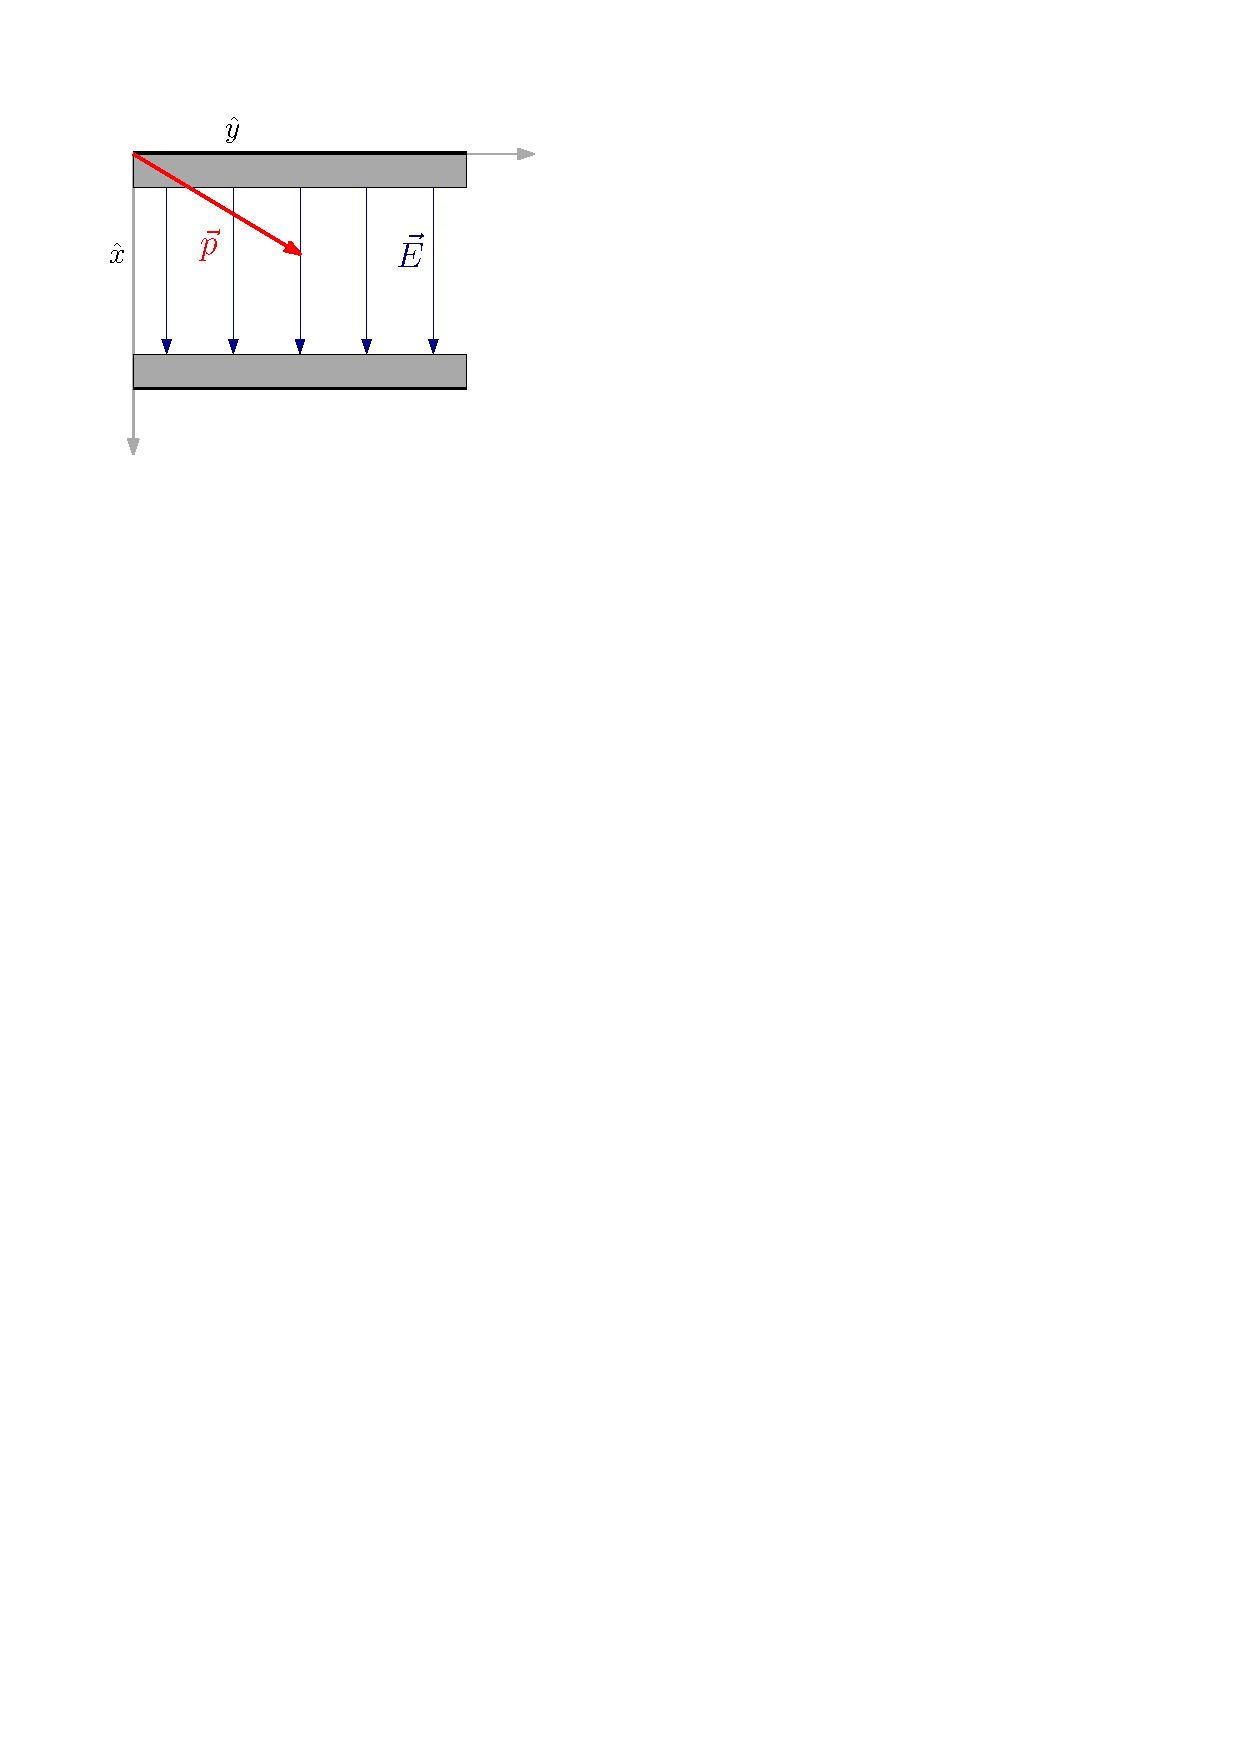
\includegraphics[scale=0.7]{Grafica/ParticellaCampoE.pdf}
    \caption{Particella carica in un campo elettrico $\vec{E}$}
    \label{motoE}
\end{figure}
Consideriamo una particella di carica unitaria $+e$ che si muove sul piano $\hat{x}\hat{y}$, con momento iniziale $\vec{p}(0) = (p_{0,x}, p_{0,y}, 0)$, in presenza di un campo elettrico uniforme e costante $\vec{E} = E\hat{x}$ lungo la direzione $+\hat{x}$.\\
Dall'espressione della forza di Lorentz (\ref{forza-lorentz}) si ottiene, visto che $\vec{B} = 0$, la seguente espressione:
\[
\frac{d\vec{p}}{dt} = e\vec{E} \Rightarrow \dot{p_x} = eE; \> \dot{p_y} = 0; \> \dot{p_z} = 0
\]
Integrando si giunge a:
\[
\begin{cases}
p_x(t) = p_{0,x}+eEt\\
p_y(t) = p_{0,y}\\
p_z(t) = 0
\end{cases}
\]
Come ci aspettavamo, il campo elettrico \textit{accelera} la particella lungo $\hat{x}$. Ammesso che il campo sia sufficientemente esteso, negli istanti precedenti a $t=0$ la particella era più lenta, e ad un certo $\bar{t}$ aveva velocità nulla lungo $\hat{x}$. Possiamo sfruttare ciò per effettuare una traslazione temporale del sistema di riferimento e rimuovere il fastidioso termine $p_{0,x}$ per semplicità di conti:
\[
t' = t+\frac{p_{0,x}}{eE} \Rightarrow t = t'-\frac{p_{0,x}}{eE} \Rightarrow p_x(t') = \hlc{Yellow}{eEt'}
\]
Per non appesantire la notazione, nei passaggi seguenti si scriverà semplicemente $p_x(t) = eEt$ eliminando gli apici.\\
Ricordando ora:
\begin{equation}
\beta = \frac{v}{c} = c\frac{p}{\mathcal{E}} \Rightarrow \frac{\vec{p}}{\mathcal{E}} = \frac{\vec{v}}{c^2} \Rightarrow \vec{v} = \frac{c^2 \vec{p}}{\mathcal{E}}
\label{velocita-momento}
\end{equation}
e la relazione di mass-shell $\mathcal{E} = \hlc{SkyBlue}{\sqrt{m^2c^4 + c^2p^2}}$, si ottiene:
\begin{align*}
    v_x = \frac{dx}{dt} = \frac{c^2 \hlc{Yellow}{p_x(t)}}{\hlc{SkyBlue}{\mathcal{E}}} = \frac{c^2 (eEt)}{\sqrt{\underbrace{m^2c^4 + 
c^2(p_{0,y}^2}_{\mathcal{E}_0} + (eEt)^2)}} = \frac{c^2 (eEt)}{\sqrt{\mathcal{E}_0^2 + c^2(eEt)^2}} = \frac{c^2(eEt)}{\mathcal{E}_0\displaystyle \left [1 + \left (\frac{c (eEt)}{\mathcal{E}_0} \right )^2\right ]^{\frac{1}{2}}}
\end{align*}
Ponendo $\alpha = eE/\mathcal{E}_0$ si giunge a:
\[
\frac{dx}{dt} = \frac{c^2 \alpha t}{\sqrt{1+(c\alpha t)^2}} = \frac{1}{\alpha}\frac{d}{dt}\sqrt{1+(\alpha c t)^2} \Rightarrow x(t) = \frac{1}{\alpha}\sqrt{1+(\alpha c t)^2} + c_x
\]
Ripetendo lo stesso conto lungo $\hat{y}$:
\[
v_y = \frac{dy}{dt} = \frac{c^2 p_y(t)}{\mathcal{E}} = \frac{c^2 p_{0,y}}{\mathcal{E}_0 \sqrt{1+(\alpha c t)^2}} = \frac{p_{0,y}c}{\mathcal{E}_0 \alpha} \frac{d}{dt} \arcsinh(\alpha c t) \Rightarrow y(t) = \frac{p_{0,y}}{\alpha\mathcal{E}_0}\arcsinh(\alpha c t) + c_y
\]
Definendo l'origine del sistema di riferimento a partire dalla posizione della particella a $t = 0$ si deducono le condizioni al contorno $x(0) = 0$ e $y(0) = 0$, che portano a trovare $c_x = -1/\alpha$ e $c_y = 0$. La traiettoria percorsa dalla particella è perciò data in forma parametrica da:
\[
\begin{cases}
x(t) = \displaystyle\frac{1}{\alpha}\left (\sqrt{1+(\alpha c t)^2} -1 \right )\\
y(t) = \displaystyle \frac{p_{0,y}c}{eE}\arcsinh(\alpha c t)
\end{cases}
\]
Da $y(t)$ si può ricavare $\alpha c t$
\[
y(t) = \displaystyle \frac{p_{0,y}c}{eE}\arcsinh(\alpha c t) \Rightarrow \frac{eEy(t)}{p_{0,y}c} = \arcsinh(\alpha c t) \Rightarrow \alpha c t = \sinh\left ( \frac{eEy(t)}{p_{0,y} c} \right )
\]
che, sostituito nell'espressione per $x(t)$, conduce alla forma grafico:
\[
x(t) = \frac{\mathcal{E}_0}{eE}\left (\sqrt{1+\sinh^2\left (\frac{eEy(t)}{p_{0,y} c}\right )} -1 \right ) = \frac{\mathcal{E}_0}{eE}\left ( \cosh\left ( \frac{eEy(t)}{p_{0,y}c} \right ) -1 \right )
\]

%[TO DO] Fare grafico
%Esamina limite a bassa velocità

\subsection{Particella carica in campo magnetico}
Consideriamo ora una particella di carica $+e$ che parte con velocità $\vec{v}(0) = (v_x(0), v_y(0), v_z(0))$ all'interno di un campo magnetico uniforme e costante $\vec{B} = (0,0,B)$ diretto lungo $+\hat{z}$.\\
Dall'espressione della forza di Lorentz (\ref{forza-lorentz}) e applicando la relazione trovata nel paragrafo precedente (\ref{velocita-momento}) si ottiene:
\begin{equation}
\frac{d\vec{p}}{dt} = \frac{\mathcal{E}}{c^2}\frac{d\vec{v}}{dt} \frac{e}{c}(\vec{v}\times\vec{B}) \Rightarrow \frac{d\vec{v}}{dt} = \frac{e c}{\mathcal{E}}(\vec{v}\times \vec{B})
\label{vel-in-B}
\end{equation}
Partendo dal risultato in (\ref{deriv-energia-E}) osserviamo poi che, essendo $\vec{E} = 0$, l'energia cinetica della particella non varia:
\[
\frac{d\mathcal{E}}{dt} = e\vec{E}\cdot \vec{v}
\]
Perciò non varia neanche il modulo della velocità, e da ciò si deduce che l'accelerazione subita dalla particella è sempre perpendicolare alla sua velocità (come nel caso classico):
\[
\frac{d\mathcal{E}}{dt} = 0 \Rightarrow \frac{dv^2}{dt} = 0 = 2\vec{v}\cdot \underbrace{\frac{d\vec{v}}{dt}}_{\vec{a}} = 0 \Rightarrow \vec{v}(t)\perp \vec{a}(t)\> \forall t
\]
Per trovare la traiettoria è necessario integrare l'equazione in (\ref{vel-in-B}). Iniziamo calcolando il termine $\vec{v}\times\vec{B}$:
\[
\vec{v}\times\vec{B} = \operatorname{det}\begin{bmatrix}
\hat{x} & \hat{y} & \hat{z}\\
v_x(t) & v_y(t) & v_z(t)\\
0 & 0 & B
\end{bmatrix} = \hat{x}(v_y(t) B) - \hat{y}(v_x(t) B)
\]
Sostituendo il risultato in (\ref{vel-in-B}) e proiettando sulle varie coordinate:
\[
\frac{dv_x}{dt} = \underbrace{\frac{ecB}{\mathcal{E}}}_{\omega}v_y; \quad \frac{dv_y}{dt} = -\underbrace{\frac{ecB}{\mathcal{E}}}_{\omega}v_x; \quad \frac{dv_z}{dt} = 0
\]
Osserviamo che, come nel caso classico, il campo magnetico lascia invariata la componente della velocità parallela ad esso. Il moto lungo $\hat{z}$ sarà perciò uniforme, e integrando si ottiene banalmente: $v_z(t) = v_z(0)$ e $x_z = z_0 + v_z(0)t$.\\
Ponendo $\omega = (ecB)/\mathcal{E}$ si giunge al sistema:
\[
\begin{cases}
\dot{v_x}(t) = \omega v_y(t)\\
\dot{v_y}(t) = -\omega v_x(t)
\end{cases}
\]
Per risolverlo definiamo la "velocità complessa" come $v_\perp(t) = v_x(t)+iv_y(t)$. Derivando e sostituendo le equazioni di sopra:
\[
\dot{v}_\perp(t) = \dot{v}_x(t) + i \dot{v}_y(t) = \omega v_y(t) - i\omega v_x(t) = -i\omega(v_x(t)+iv_y(t)) = -i\omega v_\perp(t)
\]
In questo modo si è ridotto un sistema di due equazioni differenziali a coefficienti reali in una sola (ma a coefficienti complessi), che si risolve con una semplice integrazione:
\[
\dot{v}_\perp(t) = -i\omega v_\perp(t) \Rightarrow v_\perp(t) = k e^{-i\omega t}
\]
%Questo metodo di risoluzione è esposto da Marasta a pag. 139 (appunti eq. diff. lin.)
Imponiamo quindi la condizione iniziale $v_\perp(0) = v_x(0)+iv_y(0) = k$. Osserviamo che il modulo $|v_\perp(t)| = |v_\perp(0)|$ $\forall t$, per cui $v_x(0) = |v_\perp|\cos\theta$ e $v_y(0) = |v_\perp|\sin\theta$, con $\theta = \arctan(v_y(0)/v_x(0))$.\\ %Verificare
Sostituendo nell'equazione:
\[
v_\perp(t) = |v_\perp|(\cos\theta+i\sin\theta)e^{-i\omega t} = |v_\perp|e^{-i(\omega t -\alpha)} = |v_\perp|\cos(\omega t - \alpha) - i|V_\perp|\sin(\omega t- \alpha)
\]
Per trovare le soluzioni reali per $v_x(t)$ e $v_y(t)$ basta dividere parte reale e parte immaginaria e integrare:
\[
\begin{cases}
\displaystyle v_x(t) = \frac{dx}{dt} = |v_\perp|\cos(\omega t- \alpha) =  \frac{v_\perp}{\omega}\frac{d}{dt}\sin(\omega t-\alpha)\\
\displaystyle v_y(t) = \frac{dy}{dt} = -|v_\perp|\sin(\omega t-\alpha) = \frac{v_\perp}{\omega}\frac{d}{dt}\cos(\omega t-\alpha)
\end{cases} \Rightarrow
\begin{cases}
\displaystyle x(t) - x_0 = \frac{|v_\perp|}{\omega}\sin(\omega t-\alpha)\\
\displaystyle y(t)-y_0 = \frac{|v_\perp|}{\omega}\cos(\omega t-\alpha)
\end{cases}
\]
Elevando al quadrato e sommando si elimina la dipendenza dal tempo:
\[
(x(t)-x_0)^2 + (y(t)-y_0)^2 = \frac{v_\perp^2}{\omega^2}
\]
e si trova che il moto sul piano $\hat{x}\hat{y}$ è circolare, con raggio $R=|v_\perp|/\omega$, percorso a velocità angolare uniforme $\omega$:
\[
\omega = \frac{ecB}{\hlc{Yellow}{\mathcal{E}}} = \frac{e\cancel{c}B}{\hlc{Yellow}{m\gamma c^{\cancel{2}}}} = \frac{eB}{m\gamma c} = \frac{\omega_{\text{non rel}}}{\gamma}
\]
Da cui:
\[
R = \frac{v_\perp}{\omega} = \frac{|v_\perp|}{e c B}m\gamma c^2 = \frac{|v_\perp|m\gamma c}{eB}
\]
Ricordando la relazione $|p_\perp| = \mathcal{E} |v_\perp|/c^2$ si può scrivere il raggio in funzione del momento:
\[
R = \frac{v_\perp}{\omega} = \left (\frac{c^2 p_\perp}{\mathcal{E}} \right ) \left ( \frac{\mathcal{E}}{ecB} \right ) = \frac{cp_\perp}{eB}
\]
\section{Formulario} %[TO DO] Aggiungere formule dei campi, formattare in modo che stia tutto in un A4 fronte e retro
\begin{align}
    \text{Derivata} & & \partial_\mu \equiv \frac{\partial}{\partial x^\mu} := \left (\frac{1}{c}\frac{\partial}{\partial t}, \nabla \right )\\
    & & \partial^\mu \equiv \frac{\partial}{\partial x_\mu} := \left ( \frac{1}{c}\frac{\partial}{\partial t}, -\nabla \right )\\
    \text{Quadrivelocità} & & u^\mu := \frac{dx^\mu}{ds} = \gamma(v)\left (1, \frac{\vec{v}}{c}\right ); \quad u^\mu u_\mu = 1\\
    \text{Intervallo} & & ds = \sqrt{g_{\mu\nu}dx^\mu dx^\nu} = \sqrt{dx_\mu dx^\nu} = \frac{c dt}{\gamma(v)}\\
    \text{Quadriaccelerazione} & & w^\mu := \frac{du^\mu}{ds} = \left ( \frac{\gamma^4}{c^3}\vec{v}\cdot \vec{a}, \frac{\gamma^2}{c^2}a^i + \frac{\gamma^4}{c^4}v^i(\vec{v}\cdot \vec{a}) \right ); \quad w^\mu u_\mu = 0;\\ 
    \text{Quadrimomento} & & p^\mu = mcu^\mu = \left ( \frac{E}{c}, m\gamma(v)v^i \right )\\
    \text{Energia} & & E = \sqrt{m^2c^4 + c^2|\vec{p}|^2} = m\gamma(v) c^2\\
    \text{Quadriforza} & & F^\mu = \frac{dp^\mu}{ds} = \left ( \frac{\gamma}{c^2}\vec{F}\cdot \vec{v}, \frac{\gamma}{c}\vec{F} \right ); \quad F^\mu u_\mu = 0\\
    \beta = \frac{v}{c} = c\frac{p}{E} \Rightarrow \beta = \frac{p}{E} \span \span
\end{align}

\section{Appendice}
\subsection{Cambio di variabile casuale}
Sia $x$ una variabile casuale con distribuzione data dalla pdf $f(x)$, e $y$ un'altra variabile casuale derivata dalla prima tramite una \textit{relazione funzionale} $y = T(x)$. Ci si pone il problema di trovare la pdf di $y$.\\
Il caso più semplice è se $T$ è biunivoca. Allora, intuitivamente, quando $x$ appartiene ad un intervallino centrato su $x^*$ e largo $dx$, allora $y$ si troverà in un intervallino centrato su $y^* = T(x^*)$ e largo $dy = |T'(x)|dx$ (dalla definizione di differenziale - il modulo compare poiché stiamo considerando l'ampiezza di un intervallo, quantità che è \textit{definita positiva}). Poiché $T$ è biunivoca\footnote{Nel caso $T$ non sia biunivoca sarà necessario considerare tutti gli intervallini in cui $y$ potrebbe trovarsi dato che $x$ è in $dx$, e "\textit{spalmare}" su di essi la probabilità $dp$}, tale intervallino di $y$ è \textbf{unico}. Perciò, se $x$ si trova nel suo intervallino $dx$ con probabilità $dp = f(x)dx$ (dalla def. di pdf), allora $y$ sarà \textit{per forza} in $dy$, con la stessa probabilità $dp$.\\
Poiché la $dp$ è la stessa possiamo scrivere la seguente uguaglianza:
\[
f(x)dx = g(y)dy = g(y)|T'(x)|dx \Rightarrow g(x) = \frac{f(x)}{|T'(x)|}
\]
Possiamo ora effettuare il cambio di variabili scrivendo $x$ in funzione di $y$ tramite $x = T^{-1}(y)$ (che esiste poiché $T$ è biunivoca):
\[
g(y) = \frac{f(T^{-1}(y))}{|T'(T^{-1}(y))|}
\]
che costituisce la \textbf{formula per il cambio di variabile casuale}.\\
\textbf{Esempio}. Giustifichiamo la scrittura $df(\theta) = a\sin\theta d\theta \Rightarrow dg(\cos\theta) = a\,d\cos\theta$. Qui abbiamo una variabile casuale $\theta$ che si distribuisce con pdf data da $f(\theta)$. Il cambio di variabile è $T:\theta \mapsto \cos\theta$\footnote{Nota: non è una funzione biunivoca, ma fortunatamente non sarà necessario fare considerazioni complesse grazie ad una semplificazione}. Applicando la formula:
\[
g(\cos\theta) = \frac{a \sin ( T^{-1}(\cos\theta) )}{|-\sin(T^{-1}(\cos\theta))|} = a
\]
da cui $dg(\cos\theta) = a\,d\cos\theta$ come desiderato.
\end{document}